%\documentclass[10pt,a4paper,notitlepage]{report}
\documentclass[12pt]{fithesis2}
\usepackage[utf8]{inputenc}
\usepackage[czech]{babel}
\usepackage[T1]{fontenc}

\usepackage{amsmath}
\usepackage{amsfonts}
\usepackage{amssymb}
\usepackage{amsthm}

\usepackage{float}
\usepackage{makeidx}
\usepackage{graphicx}
\usepackage{syntax}    % texlive-mdwtools
\usepackage{csquotes}
\usepackage{glossaries}
\usepackage{todonotes} % command \todo
\usepackage[plainpages=false,pdfpagelabels]{hyperref}
\usepackage{listings}

\usepackage{pdfpages}
\usepackage[toc,page,title,titletoc]{appendix}
\usepackage[
   backend=biber      % if we want unicode 
  ,style=iso-numeric % or iso-numeric for numeric citation method          
  ,autolang=other        % to support multiple languages in bibliography
  ,sortlocale=cs_CZ   % locale of main language, it is for sorting
  ,bibencoding=UTF8   % this is necessary only if bibliography file is in different encoding than main document
]{biblatex}

\thesistitle{Partial Order redukce pro LLVM} % enter thesis title
\thesissubtitle{Bakalářská práce}
\thesisstudent{Jan Tušil}
\thesiswoman{false}
\thesisfaculty{fi}
\thesisyear{jaro 2015}
\thesisadvisor{Mgr. Petr Bauch} % fill in advisor’s name
\thesislang{cz}

\floatstyle{boxed}
\restylefloat{figure}
\addbibresource{literature.bib}

\author{Jan Tušil <410062@mail.muni.cz>}
\title{LLVM PO}

\newtheorem{definition}{Definice}
\newtheorem{lemma}     {Lemma}
%\newtheorem{proof}     {Důkaz}
\newtheorem{decision}  {Rozhodnutí}

\newcommand{\tuple}[1]{\langle #1 \rangle}
\newcommand{\suchthat}{\mid}

\renewcommand{\appendixname}{Priloha}

% převzato z http://tex.stackexchange.com/a/5809
\newcommand\fnurl[2]{%
  \href{#2}{#1}\footnote{\url{#2}}%
}

\hyphenation{vstup-ní}
\hyphenation{nu-me-ri-cal}
\hyphenation{pře-cho-do-vý-mi}
\hyphenation{fun-kce}
\hyphenation{snad-no}
\hyphenation{pro-měn-nou}
\hyphenation{ana-ly-zé-ru}
\hyphenation{něk-te-ré}

\lstset{ %
%  backgroundcolor=\color{white},   % choose the background color; you must add \usepackage{color} or \usepackage{xcolor}
  basicstyle=\footnotesize
}


\begin{document}

\FrontMatter
\ThesisTitlePage

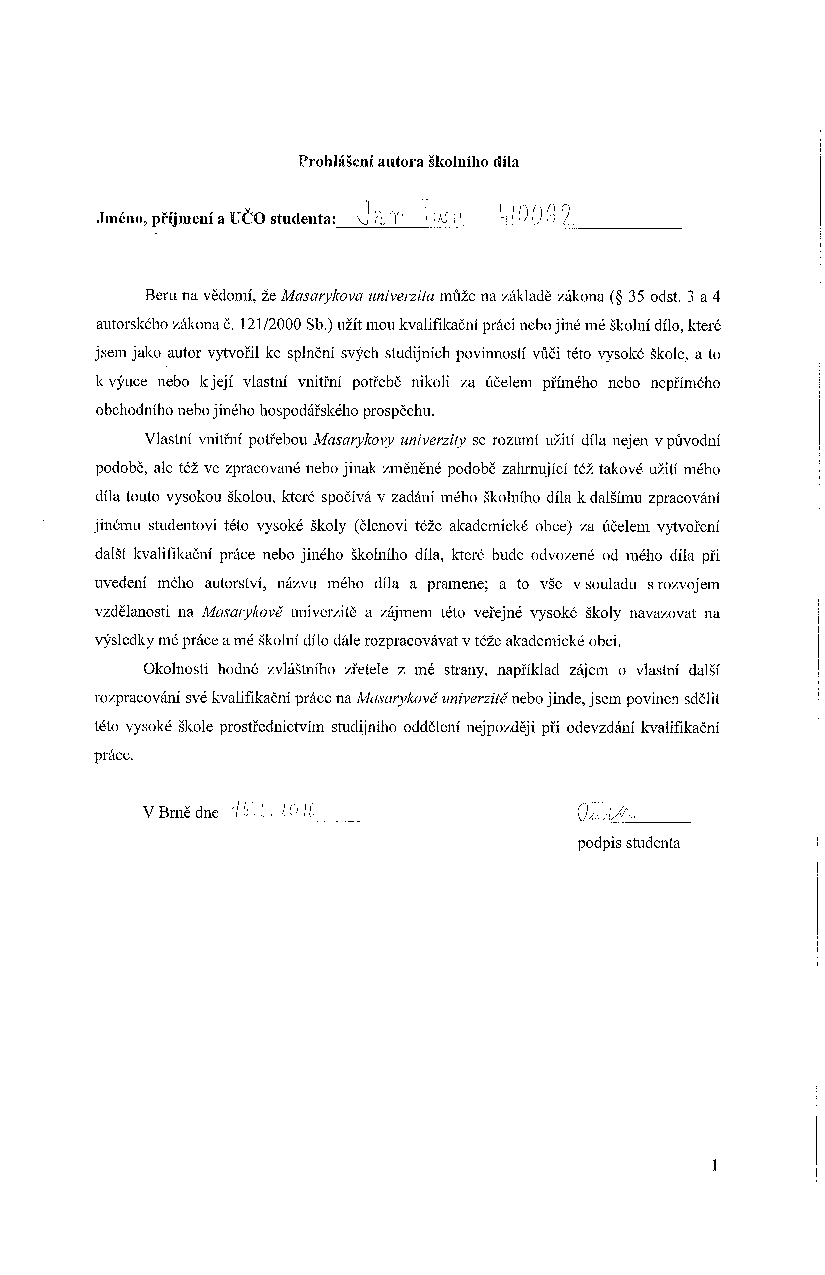
\includepdf[pages={1}]{prohlaseni.pdf}
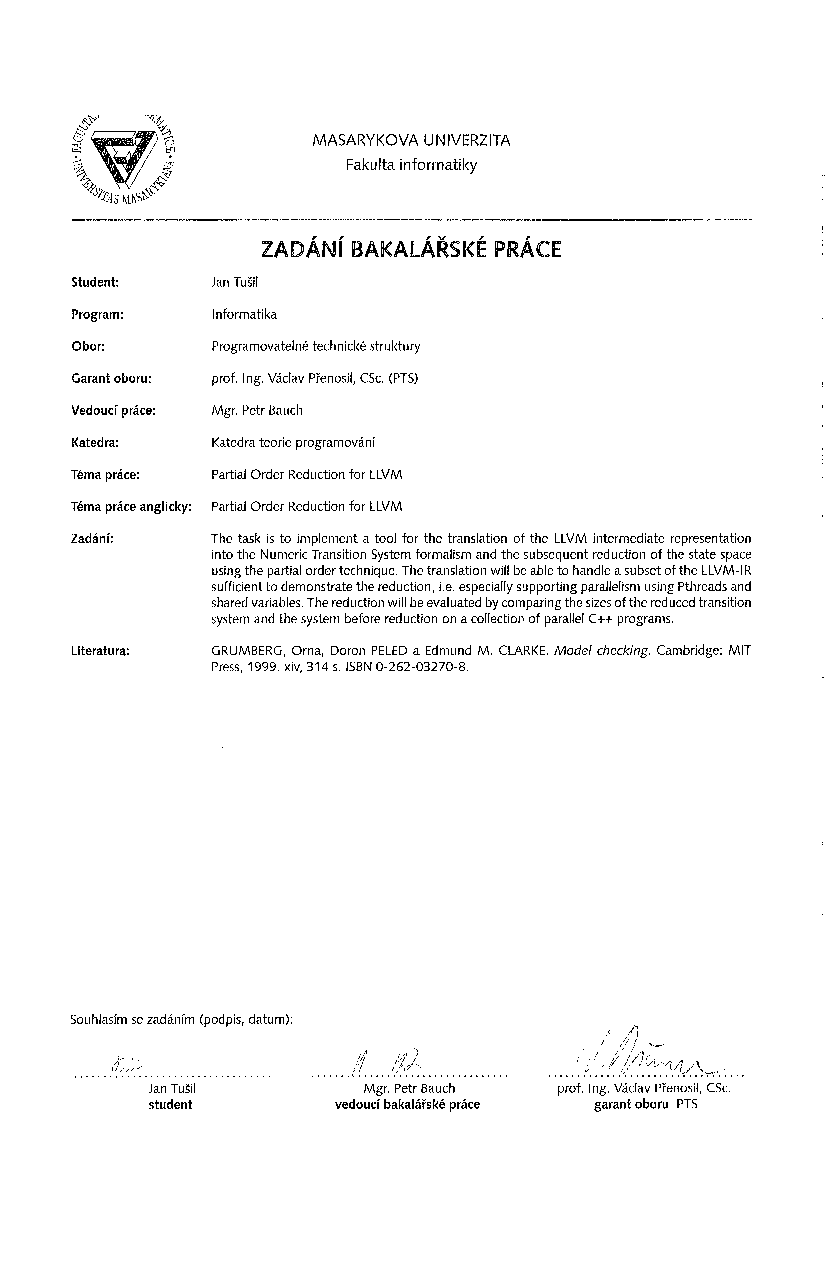
\includepdf[pages={1}]{zadani.pdf}



\begin{ThesisDeclaration}
\DeclarationText
\AdvisorName
\end{ThesisDeclaration}

\begin{ThesisThanks}
I would like to thank my supervisor...
\end{ThesisThanks}

\begin{ThesisAbstract}
Cílem této bakalářské práce je umožnit analýzu a verifikaci paralelních programů využívajících pthreads v jazyce LLVM IR nástrojům, jež dokáží pracovat s přechodovými systémy v jazyce NTS. Za tímto účelem práce implementuje statickou verzi techniky zvané \textit{Partial Order Reduction}.
\end{ThesisAbstract}
\begin{ThesisKeyWords}
model checking, partial order reduction, LLVM, NTS
\end{ThesisKeyWords}
\MainMatter

\tableofcontents

\chapter{Úvod}
\section{Motivace}
Model checking~\cite{CLARKE} (česky ověřování modelu) je v současné době oblíbenou technikou pro automatizovanou formální verifikaci softwaru i hardwaru, trpí však problémem stavové exploze zejména při verifikaci paralelního softwaru. Jednou z možností jak zmenšit počet stavů, které je třeba ověřit, je použití techniky nazývané (z historických důvodů~\cite{CLARKE}) Partial Order Reduction (redukce částečným uspořádáním, POR), která využívá komutativity některých paralelně vykonávaných instrukcí.

Jazyk LLVM IR je součástí projektu LLVM~\cite{LLVM}, jehož cílem je vytvoření infrastruktury pro tvorbu překladačů. V současné době existují nástroje~\cite{LLBMC} určené pro model checking jazyka LLVM, ne všechny z nich~\cite{BBH+13} však implementují POR. Cílem této práce je vytvořit z programu v jazyce LLVM IR využívajícím posixová vlákna (pthreads) odpovídající redukovaný sekvenční přechodový systém v jazyce NTS.

\section{Přístup}
Tuto úlohu je možné přirozeně rozdělit na dvě části, a to na
\begin{enumerate}
\item přirozený překlad programu z LLVM IR do NTS se zachováním paralelismu (část dále označovaná jako překlad), a
\item převod paralelního programu v jazyce NTS na sekvenční program s využitím POR (část dále označovaná jako sekvencializace).
\end{enumerate}
Tyto dvě části jsou poměrně nezávislé a mohou být implementovány jako rozdílné nástroje, pracující nad společnou knihovnou. Rozdělením navíc získáváme možnost ověřovat vlastnosti sekvenčních programů v jazyce LLVM IR nástrojem, který rozumí jazyku NTS.

% Related work: Petrův parser.

%Všechno ve formě knihovny - jednoduché rozhraní, snadno použitelné.

\section{Popis následujících kapitol}
Následující text obsahuje nejprve popis použitých technologií (kap.~\ref{sec:technologies}), konkrétně jazyka LLVM IR, knihovny posixových vláken, jazyka NTS a techniky POR, následuje krátká analýza (kap.~\ref{sec:analysis}) řešeného problému a popis způsobu překladu jazyka LLVM IR do jazyka NTS (kap.~\ref{sec:translation}). Další kapitola~(\ref{sec:nts-por}) obsahuje komentář k použití POR pro redukci přechodových systému v jazyce NTS, následovaná kapitolou~\ref{sec:implementation} zabývající se implementací knihovny \textit{libNTS}, která slouží k práci s paměťovou reprezentací přechodového systému v jazyce NTS. Práci uzavíráme krátkým popisem experimentálních výsledků.


%%%%%%%%%%%%%%%%%%%%%%%%%%%%%%%%%%%%%%%%%%%%%%%%%%%%%%%%%%%%%%%%%%%%%%%%%%%%%%%%

\chapter{Použité technologie}
\label{sec:technologies}
\section{LLVM}
Projekt LLVM~\cite{LLVM} je sada knihoven a nástrojů, tvořící infrastrukturu pro tvorbu překladačů. Ke své činnosti využívá mezijazyk známý jako LLVM intermediate representation~\cite{LLVM-langRef} (dále LLVM IR nebo jen IR) a sadu dobře definovaných softwarových rozhraní pro manipulaci s~ním. Práci překladače vybudovaného nad LLVM lze rozdělit do několika fází: nejprve je zpracován kód ve vstupním jazyce (proběhne lexikální, syntaktická a sémantická analýza), poté je vygenerován mezikód v~jazyce LLVM IR, nad tímto pak proběhnou zvolené optimalizace, z~výsledného IR kódu je vygenerován platformově specifický kód a~proběhne linkování. Tato architektura umožňuje využít při tvorbě překladače již jednou napsaných částí~\cite{AOSABOOK-LLVM}.

\subsection{LLVM IR}
LLVM IR je typovaný jazyk podobný jazyku symbolických adres, od kterého se však liší v několika zásadních vlastnostech.
\begin{itemize}
\item LLVM IR je platformově nezávislý a není určený pro žádný fyzicky existující procesor.
\item V jazyce LLVM IR je možné používat neomezené množství registrů.
\item Do každého registru je možné přiřadit hodnotu pouze jednou. Tato vlastnost je nazývána \textit{static single assignment form} (dále \textit{SSA}).
\end{itemize}
Kód je uchováván v~modulech a~rozčleněn do funkcí, které se skládají ze základních bloků. Základní blok (basic block) je taková posloupnost instrukcí, která má jeden vstupní bod a~jeden výstupní. Zejména tedy není možné provádět skoky dovnitř bloku nebo vyskočit z~bloku jinde, než na konci. Sémantika tohoto jazyka je dobře zdokumentována, navíc probíhá práce na její formalizaci~\cite{LLVMForm}.

\subsubsection{Instrukční sada}
Instrukční sada LLVM IR je svou jednoduchostí podobná RISCovým instrukčním sadám. Instrukce jsou rozděleny na ukončovací, binární, bitové, paměťové a ostatní, přičemž pouze ukončovací instrukce mohou měnit tok řízení. Tyto instrukce vždy ukončují základní blok a rozhodují, který blok bude vykonán po dokončení aktuálního.

\subsubsection{Příklad}
Obrázek \ref{IR-EX} zobrazuje funkci, vygenerovanou nástrojem clang~\cite{clang} z~kódu v~jazyce C. Funkce je globálním symbolem (globální symboly mají prefix \texttt{@}), má návratovou hodnotu \texttt{i32} (dvaatřicetibitové celé číslo) a~jako parametr přijímá proměnnou téhož typu. V~těle funkce se vyskytuje pouze jedna ukončovací instrukce, totiž \texttt{ret}, a~celá funkce je tak tvořena jedním základním blokem. Symbol \texttt{\%1} označuje výsledek instrukce \texttt{alloca}, což je lokální proměnná typu ukazatel na \texttt{i32} (lokální symboly mají prefix \texttt{\%}). Následuje instrukce \texttt{store}, která zkopíruje hodnotu parametru \texttt{\%x} na právě alokované paměťové místo a~nevrací žádnou hodnotu. Po načtení hodnoty z~paměti a~přičtení jedničky je vrácen výsledek poslední operace.


\begin{figure}[h!]
\begin{lstlisting}
define i32 @add(i32 %x) #0 {
%1 = alloca i32, align 4
store i32 %x, i32* %1, align 4
%2 = load i32* %1, align 4
%3 = add nsw i32 1, %2
ret i32 %3
}
\end{lstlisting}
\caption{Ukázka IR kódu}
\label{IR-EX}
\end{figure}

\subsection{Průchody}
Průchod (orig. pass) je softwarový modul, který pracuje nad kódem v~LLVM IR. Průchody se dají rozdělit na analytické a transformační: analytické kód nijak nemodifikují, ale počítají nějakou užitečnou informaci; transformační ze vstupního kódu generují jiný. Typickým příkladem transformačního průchodu je eliminace mrtvého kódu (dead code elimination, DCE). Nástroj využívající LLVM si může zvolit, které průchody budou spuštěny; také je možné spouštět je ručně pomocí nástroje opt, dodávaného spolu s~LLVM.

\subsection{Využití}
V současné době existují nástroje pro software model checking (model checkery), které přijímají model v~jazyce LLVM IR. Mezi ně patří například DIVINE~\cite{BBH+13}. Využití tohoto jazyka přináší celou řadu výhod. Zaprvé, pro velké množství překladačů do LLVM IR je model checker méně závislý na programovacím jazyku, v~němž je napsaný ověřovaný software. Dále, před vlastní model checking lze zařadit již napsané průchody, které nástroji poskytnou užitečné informace nebo zrychlí model checking samotný.

%\subsubsection{Vztah k této práci}
%Z uvedených důvodů budeme i~v~této práci jako vstupní jazyk využívat právě LLVM IR. Nicméně protože sémantika tohoto jazyka není definovaná formálně a~v~oblasti model checkingu se obvykle pracuje s~přechodovými systémy (jako jsou Kripkeho struktury~\cite{CLARKE}), v~této práci bude výhodné pracovat s~jazykem popisujícím přechodový systém.


\section{Posix threads}
\label{sec:posix-threads}
Jazyk LLVM IR sám neposkytuje podporu pro explicitní paralelismus. Té je možné docílit pouze použitím specializovaných knihoven. Knihovna Posix threads (zkráceně pthreads) je standardizovanou knihovnou s rozhraním pro jazyk C, která obsahuje funkce pro manipulaci s vlákny.

\subsection{pthread_create()}
Nejzajímavější funkcí z této knihovny je \texttt{pthread\_create}\cite{man-pthread-create} (viz obrázek~\ref{fig:pthread-create-c}), která spustí funkci, jež dostala jako argument parametru \texttt{start\_routine}, v nově vytvořeném vlákně. Funkce dále uloží ID vlákna do proměnné \texttt{*thread} (nesmí být \texttt{null}), argument parametru \texttt{arg} předá jako parametr funkci \texttt{start\_routine} a o úspěchu či neúspěchu informuje volajícího prostřednictvím návratové hodnoty.

Protože podle normy POSIX.1-2001 \cite{posix} je \texttt{pthread\_t} neprůhledný (opaque) datový typ, prototyp této funkce v jazyce LLVM IR je platformově závislý. Na obrázku~\ref{fig:pthread-create-llvm} se nachází prototyp \texttt{pthread\_create}, jak je k dispozici v systému Fedora 21 x86_64 s GNU libc verze 2.20 (pthreads jsou součásti glibc).

\begin{figure}[h!]
\begin{lstlisting}[language=C]
int pthread_create (pthread_t *thread,
                    const pthread_attr_t *attr,
                    void *(*start) (void *),
                    void *arg                   );
\end{lstlisting}
\label{fig:pthread-create-c}
\caption{Prototyp funkce \texttt{pthread_create} v jazyce C}
\end{figure}

\begin{figure}[h!]
\begin{lstlisting}[language=llvm]
declare i32 @pthread_create (
	i64*, %union.pthread_attr_t*,
	i8* (i8*)*, i8*               )
\end{lstlisting}
\label{fig:pthread-create-llvm}
\caption{Prototyp funkce \texttt{pthread_create} v jazyce LLVM IR}
\end{figure}

\section{NTS}
Jazyk NTS (Numerical Transition Systems) je jednoduchý jazyk s~formalizovanou sémantikou, sloužící pro popis numerických přechodových systémů. NTS mohou modelovat libovolný software~\cite{NTSref} a~protože software je obvykle strukturován do menších částí, NTS obsahuje konstrukce pro hierarchickou i~paralelní kompozici systémů. Následuje stručný popis tohoto jazyka, zájemci o preciznější popis mohou nahlédnout do~\cite{NTSref}.

\subsection{BasicNts}
Základní jednotkou NTS je BasicNts, což je samostatný přechodový systém, sestávájící z proměnných, řídících stavů a přechodů mezi nimi. Řídící stavy mohou být označeny jako iniciální, finální a chybové. Přechody jsou tvaru $s_i \overset{R}{\rightarrow} s_j$, kde $R$ je přechodové pravidlo, strážící přechod, a $s_i, s_j$ řídící stavy. Přechod může být vykonán pouze v případě, že je přechodové pravidlo naplněno.

\subsection{Proměnné}
Kromě lokálních proměnných nějakého BasicNts může přechodový systém obsahovat i proměnné globální. Jazyk navíc obsahuje speciální konstrukci pro proměnné, které se za běhu nemění: takové jsou nazývány \textit{parametry}.

\subsection{Přechodová pravidla}
Přechodová pravidla mohou být dvojího druhu: volací pravidlo (například  $(p1',p2') = \texttt{factorize} (x)$) slouží k zavolání jiného BasicNts, předání parametrů volanému a uložení výsledků volání, zatímco formulové pravidlo (například $d' * d' = x$) obsahuje formuli predikátové logiky prvního řádu, jejíž splnění umožňuje přechod do cílového stavu přechodu. 

\subsection{Formule}
Formule mohou být kvantifikované a jsou složeny pomocí logických spojek z atomických propozic a jiných formulí, přičemž za atomické propozice jsou považovány zejména booleovské termy a výsledky porovnání termů, navíc také \texttt{havoc} (viz~\ref{subsec:nts-havoc}). Nutno poznamenat, že ve formuli se mohou vyskytovat i hodnoty proměnných, platné v cílovém stavu. Tyto jsou označené znakem $'$. Jak je vidět u předchozího příkladu, je tak možné vytvořit formuli, která požaduje, aby hodnota proměnné $y$ v příštím stavu byla odmocninou hodnoty proměnné $x$ ve stavu současném.

\subsection{Termy}
Termy jsou již na syntaktické úrovni rozděleny na aritmetické a booleovské. Mezi booleovské termy patří booleovské konstanty, booleovské proměnné a jiné termy, pospojované obvyklými logickými operacemi. Obdobně, aritmetické termy jsou reálné a celočíselné konstanty a proměnné, pospojované aritmetickými operacemi z množiny $\{+, -, *, /, \% \}$. Jazyk explicitně vyžaduje, aby všechny subtermy každého termu měly stejný datový typ, jako celý term.

\subsection{Typový systém}
Jazyk NTS je vybaven třemi skalárními datovými typy: \texttt{Int}, \texttt{Bool}, \texttt{Real}. Datový typ \texttt{Int} reprezentuje matematické celé číslo, jeho doménou je tedy množina $\mathbb{Z}$; datový typ \texttt{Real} reprezentuje matematické reálné číslo, tedy jeho doménou je množina $\mathbb{R}$; nakonec typ \texttt{Bool} nabývá pouze hodnoty z množiny $\{ \texttt{true}, \texttt{false} \}$. Jazyk dále podporuje typ pole hodnot libovolného skalárního aritmetického typu.

\subsection{Sémantika}
\label{subsec:nts-configuration}

% Transition rule maps some configuration to another configuration
\newcommand{\rulemapsto}[1]{\overset{#1}{\mapsto}}
Konfigurací systému se nazývá dvojice $\tuple{q, v}$, kde $q$ je jedním z řídících stavů a $v$ valuace proměnných (tedy funkce, která každé proměnné přiřazuje hodnotu). Přechod z~konfigurace $c_1 = \tuple{q_1, v_1}$ do konfigurace $c_2 = \tuple{q_2, v_2}$ je možný, pokud existuje přechodové pravidlo $t = \left({q_1 \overset{F}{\rightarrow} q_2}\right)$ s~následující vlastností: formule vzniklá z~$F$ nahrazením proměnných $p$ hodnotami $v_1(p)$ a~nahrazením proměnných ve tvaru $p'$ hodnotami $v_2(p)$ je tautologií. Tuto situace budeme zapisovat jako $c_1 \rulemapsto{t} c_2$. Formálnější popis je k~dispozici v~\cite{NTSref}.

\subsection{Havoc}
\label{subsec:nts-havoc}
Účelem atomické propozice \texttt{havoc} je zamezit samovolné modifikaci proměnných neuvedených ve formuli přechodového pravidla. Ve své podstatě se jedná o syntaktickou zkratku.
\begin{equation}
\texttt{havoc} \left( v_1, v_2, \ldots, v_k \right) = \bigwedge_{v \in V \setminus \{ v_1, v_2, \ldots, v_k \}} v = v'
\end{equation}
Její význam si můžeme ukázat na následujícím příkladu: uvažme přechodový systém s proměnnými $x,y$ typu int, konfiguraci $s_1 = \tuple{q_1, v_1} \land v_1(x) = 0 \land v_1(y) = 3$, konfiguraci $s_2 = \tuple{q_2, v_2} \land v_2(x) = 1 \land v_2(y) = 5$ a přechod $q_1 \overset{F}{\rightarrow} q_2$. Pokud $F \equiv x' = x + 1$, pak je možné s využitím uvedeného pravidla přejít z konfigurace $q_1$ do konfigurace $q_2$, protože formule $1 = 0 + 1$ je tautologií. Tento přechod ale v rozporu s očekáváním modifikuje proměnnou y. Naopak, pokud $F \equiv x' = x + 1 \land \texttt{havoc}(x)$, potom uvedené pravidlo nelze použít pro přechod z $q_1$ do $q_2$. Po dosazení a expandování \texttt{havoc} totiž vznikne formule $1 = 0 + 1 \land 3 = 5$, která je nesplnitelná.

\subsection{Paralelismus}
\label{subsec:nts-paralelism}
Jazyk NTS umožňuje paralelní běh libovolného konečného počtu vláken. Ke každému vláknu je přiřazen \textit{vstupní bod} (entry point), což je BasicNts, který je vykonáván v kontextu daného vlákna. Paralelní NTS obsahuje specifikaci, tvořenou seznamem dvojic \texttt{vstupní bod [ počet vláken ]}. Identifikátory vláken jsou vláknům přiřazeny vzestupně od nuly, a to ve stejném pořadí, v jakém jsou zadány ve specifikaci.  Uvážíme-li příklad \ref{fig:nts-instances}, paralelní NTS obsahuje $N+1$ vláken, přičemž vstupním bodem vláken s $\texttt{tid} \in \{ 0, \ldots, N - 1 \}$ je \texttt{worker\_nts} a vstupním bodem vlákna s $\texttt{tid} = N$ je \texttt{main\_nts}.

\begin{figure}[h!]
\begin{lstlisting}
instances worker_nts[N], main_nts[1];
\end{lstlisting}
\caption{Specifikace paralelně vykonávaných vláken v jazyce NTS}
\label{fig:nts-instances}
\end{figure}



\subsection{Příklad}
Na obrázku~\ref{fig:nts-prodcons} se nachází příklad jednoduchého paralelního systému s jedním producentem a jedním konzumentem, reprezentovanými BasicNts \texttt{producent} a \texttt{consument}. Po deklaraci globálních proměnných \texttt{G} a \texttt{c} je uvedena formule, kterou musí splňovat iniciální konfigurace  (viz~\ref{subsec:nts-configuration}) paralelního systému. Systém bude obsahovat dvě vlákna, přičemž vlákno s $\texttt{tid} = 0$ bude vykonávat kód BasicNts \texttt{producent} a vlákno s $\texttt{tid} = 1$ bude vykonávat kód \texttt{consument}.

BasicNts \texttt{producent} obsahuje lokální proměnnou \texttt{i}, která je přechodem z iniciálního stavu \texttt{si} nastavena na hodnotu $0$ a každým dalším přechodem inkrementována. Přechod $\texttt{sl} \rightarrow \texttt{sl}$ se může uskutečnit pouze v případě, že globální proměnná \texttt{c} je nastavena na  hodnotu \texttt{false}, a sám tuto proměnnou nastaví na \texttt{true}. Naopak, přechod $\texttt{sl} \rightarrow \texttt{sl}$ v \texttt{consument} může být vykonán pouze v případě, že $\texttt{c} = \texttt{true}$. Činnost celého systému je taková, že \texttt{producent} postupně do proměnné \texttt{G} ukládá zvyšující se hodnoty, které \texttt{consument} sčítá.

Mimochodem, již zmíněný přechod $\texttt{sl} \rightarrow \texttt{sh}$ v \texttt{consument} ničí hodnotu uloženou v \texttt{G}, což ale nevadí, protože \texttt{G} není nikdy čtena.

\begin{figure}[t]
\begin{lstlisting}
G : int;
c : bool;
init G = 0 && l = false;
instances producent[1], consument[1];

producent {
    initial si;
    i : integer;
    si -> sl { i' = 0 && havoc(i)          }
    sl -> sl { c  = false && c' = true  &&
               G' = i     && i' = i + 1 &&
               havoc(c, G, i)              }
}

consument {
	initial si;
	sum, x : integer;
	si -> sl { sum' = 0 && havoc( sum )          }
	sl -> sh { c = true && x' = G && havoc(x, G) }
	sh -> sl { sum' = sum + x && c' = false &&
	           havoc(sum, c)                     }
}

\end{lstlisting}
\caption{Příklad kódu v jazyce NTL}
\label{fig:nts-prodcons}
\end{figure}

\section{Partial Order Reduction}
\label{sec:POR}
Partial Order Reduction je technika pro redukci stavového prostoru (paralelních) programů, která využívá komutativity paralelně vykonávaných přechodů. Pokud lze efektivně ověřit, že stav programu po vykonání přechodů $t_1$ a $t_2$ nezávisí na jejich pořadí a ověřovaná vlastnost není citlivá na volbu jednotlivých přechodů, není třeba uvažovat některé dosažitelné stavy. Technika použitá v této práci vychází z techniky popsané v \cite{CLARKE}, úprava POR pro jazyk NTS je popsána v kapitole~\ref{sec:nts-por}.

\subsection{Přechodový systém}
\textit{Stavový přechodový systém} je čtveřice $\tuple{S, T, S_0, L}$, kde $S$ představuje množinu stavů, $T \subseteq \mathcal{P}\left({S \times S}\right)$ množinu přechodových relací (dále zkráceně jen přechodů), $S_0 \in S$ označuje iniciální stav a $L : S \rightarrow \mathcal{P}\left({\mathit{AP}}\right)$ je značkovací funkce, která každému stavu přiřazuje množinu atomických propozic. Jako syntaktickou zkratku za $\tuple{s_1, s_2} \in \alpha$, kde $\alpha \in T$, zavádíme $s_1 \xrightarrow{\alpha} s_2$.

Přechod $\alpha \in T$ se nazývá deterministický, pokud pro každý stav $s \in S$ existuje nejvýše jeden stav $s' \in S$ takový, že $s \xrightarrow{\alpha} s'$ je splněno. Pro takový přechod můžeme zkráceně psát $s' = \alpha(s)$. Zatímco v \cite{CLARKE} jsou uvažovány pouze přechodové systémy s deterministickými přechody, v této práci uvažujeme přechody obecně nedeterministické.

%Vyžadujeme, aby prvky \mathit{T} musí být vzájemně disjunktní, tedy aby mezi každou dvojicí stavů existoval nejvýše jeden přechod\footnote{Tento požadavek v \cite{CLARKE} chybí.}.

\begin{definition}
Přechod $\alpha \in T$ je povolený ve stavu $s \in S$ (píšeme $\alpha \in \mathit{enabled}(s)$ právě tehdy, když existuje stav $s'$ tak že $s \xrightarrow{t} s'$.
\end{definition}

\begin{definition}
Cesta ze stavu $s_0$ v přechodovém systému je (potenciálně nekonečná) posloupnost $s_0 \xrightarrow{\alpha_0} s_1 \xrightarrow{\alpha_1} \ldots $ taková, že $\forall i \ldotp \left({ s_i \xrightarrow{\alpha_i} s_{i+1} }\right)$.
\end{definition}

\subsection{Nezávislost a komutativita přechodů}

\begin{definition}
Binární relaci $I \subseteq T \times T$ nazýváme relací nezávislosti, pokud je symetrická, antireflexivní a pro libovolnou dvojici přechodů $\tuple{\alpha, \beta} \in I$ povolených ve stavu $s \in S$ platí:
\begin{equation}\label{eq:independent-my}
\begin{split}
&\forall s_2 \in S \ldotp
\left({
	s \xrightarrow{\beta} s_2
	\Rightarrow
	\alpha \in \mathit{enabled}\left({s_2}\right)
}\right)
\land \\
&\forall s_2, s_3 \in S \ldotp \left({
	s_1 \xrightarrow{\beta} s_2 \xrightarrow{\alpha} s_3
	\Rightarrow
	\exists s_2' \in S \ldotp \left({
		s \xrightarrow{\alpha} s_2' \xrightarrow{\beta} s_3
	}\right)
}\right)
\end{split}
\end{equation}

\end{definition}


Odpovídající definice v \cite{CLARKE} požaduje (kromě symetrie a antireflexivity), aby pro každou dvojici přechodů $\tuple{\alpha, \beta} \in I$ povolených ve stavu $s \in S $ platilo:
\begin{equation}\label{eq:independent-clarke}
\alpha \in \mathit{enabled}\left({ \beta\left({s}\right) }\right) \land
\alpha\left({\beta\left({s}\right)}\right) = \beta\left({\alpha\left({s}\right)}\right)
\end{equation}

\begin{lemma}
Pro přechodové systémy bez nedeterministických přechodů jsou obě definice ekvivalentní.
\end{lemma}

\begin{proof}
Formule~\ref{eq:independent-my} i~\ref{eq:independent-clarke} se vyjadřují o stejné množině přechodů, pro důkaz lemmatu stačí dokázat ekvivalenci těchto formulí pro deterministické přechody. Protože $\beta \in \mathit{enabled}(s)$ je deterministická, existuje právě jeden stav $s_2$ takový, že $s \xrightarrow{\beta} s_2$, a to $s_2 = \beta\left({s}\right)$. Formuli~\ref{eq:independent-my} tedy můžeme přepsat jako

\begin{equation}
\begin{split}
& \alpha \in \mathit{enabled}\left({\beta\left({s}\right)}\right)
\land \\
&\forall s_3 \in S \ldotp \left({
	\beta\left({s}\right) \xrightarrow{\alpha} s_3
	\Rightarrow
	\exists s_2' \in S \ldotp \left({
		s \xrightarrow{\alpha} s_2' \xrightarrow{\beta} s_3
	}\right)
}\right)
\end{split}
\end{equation}
Protože požadujeme $\alpha \in \mathit{enabled}\left({\beta\left({s}\right)}\right)$ a uvažujeme pouze deterministické přechody, opět existuje pouze jeden takový stav $s_3$, a to $s_3 = \alpha{\left({\beta\left({s}\right)}\right)}$. Vhodný stav $s_2'$ také může být pouze jeden, a to právě $\alpha\left({s}\right)$. Formuli můžeme opět zjednodušit na
\begin{equation}
\alpha \in \mathit{enabled}\left({\beta\left({s}\right)}\right)
\land
\alpha\left({s}\right) \xrightarrow{\beta} \alpha{\left({\beta\left({s}\right)}\right)}
\end{equation}
a protože relace $I$ je symetrická, musí také platit $\beta \in \mathit{enabled}\left({\alpha\left({s}\right)}\right)$, tedy výraz $\beta\left({\alpha\left({s}\right)}\right)$ je dobře definovaný, díky čemuž můžeme formuli zjednodušit do podoby
\begin{equation}
\alpha \in \mathit{enabled}\left({\beta\left({s}\right)}\right)
\land
\beta\left({\alpha\left({s}\right)}\right) = \alpha{\left({\beta\left({s}\right)}\right)}
\end{equation}
ve které je ekvivalence s \ref{eq:independent-clarke} zřejmá.
\end{proof}



Technika, použitá v \cite{CLARKE}, tedy partial order reduction s využitím dostatečných (ample) množin, spočívá v tom, že pro každý dosažitelný stav je spočítána množina přechodů $\mathit{ample}(s) \subseteq \mathit{enabled}(s)$, která má tu vlastnost, že přechody mimo $\mathit{ample}(s)$ nejsou ,,důležité''. Formálněji řečeno je třeba, aby ke každé cestě z iniciálního stavu přechodového systému existovala vhodným způsobem ekvivalentní\footnote{Jedná se o ,,koktavou'' (stuttering) ekvivalenci, viz \cite{CLARKE}.} cesta z téhož stavu, která nevyužívá žádné přechody mimo $\mathit{ample}$. Při procházení přechodového grafu pak není třeba uvažovat přechody mimo $\mathit{ample}$, což zmenšuje počet stavů, které je nutné prozkoumat během model checkingu. Dosažitelnost stavu je přitom řešena pomocí algoritmu prohledávání do hloubky (dále DFS) z iniciálního stavu.

\begin{definition}
Přechod je neviditelný, pokud nikdy nezmění platnost atomické propozice z množiny předem vybraných propozic.
\end{definition}

\subsection{Nutné podmínky}
\label{subsec:por:ample-conditions}
Kniha~\cite{CLARKE} uvádí několik podmínek, postačujících pro volbu vhodného $\mathit{ample}(s)$.

\begin{enumerate}
\item[C0] $\mathit{ample}(s) = \emptyset \Rightarrow \mathit{enabled}(s) = \emptyset$
\item[C1] Každá cesta v úplném explicitním přechodovém grafu paralelního systému, začínající ve stavu $s$, má následující vlastnost: pokud přechod $\beta$, který se vyskytuje po cestě, závisí na nějakém přechodu $\alpha \in \mathit{ample}(s)$, pak se před jeho výskytem vyskytuje nějaký přechod $\alpha' \in \mathit{ample}(s)$.
\item[C2] Pokud $s$ není plně expandovaný, pak každý přechod z $\mathit{ample}(s)$ je neviditelný.
\item[C3] Nesmí existovat cyklus, který obsahuje přechod povolený v některém z jeho stavů a neobsažený v žádném z $\mathit{ample}$ stavů cyklu.
\end{enumerate}

\subsection{Výpočet ample(s)}
\label{subsec:por-compute-ample}
Pro splnění C3 stačí, aby v každém cyklu existoval alespoň jeden plně expandovaný stav, C2 je možné ověřit přímo z definice neviditelnosti přechodu. Ověřit podmínku C1 tak snadné není; \cite{CLARKE}~dokonce uvádí, že problém ověření podmínky C1 pro jeden stav je alespoň tak těžký, jako problém dosažitelnosti stavu v celém přechodovém systému. Z tohoto důvodu byly navrženy heuristiky, jejichž cílem je pro stav $s$ efektivně zvolit $ample(s)$ tak, aby byly podmínky (nebo alespoň podmínka C1) jistě splněny. Tyto heuristiky silně závisí na použitém modelu výpočtu a proto budou v tomto textu popsány až v sekci~\ref{sec:nts-por} přímo pro jazyk NTS.

%%%%%%%%%%%%%%%%%%%%%%%%%%%%%%%%%%%%%%%%%%%%%%%%%%%%%%%%%%%%%%%%%%%%%%%%%%%%%%%%

%BTW: NTS je 'ten' - system
\chapter{Analýza problému}
\label{sec:analysis}
Jak již bylo řečeno v úvodu, celá úloha se skládá ze dvou částí, tedy z překladu programu z LLVM IR do NTS a  ze sekvencializace vytvořeného paralelního NTS s použitím POR. Pokud bychom o přeloženém paralelním NTS nic nepředpokládali, nástroj pro sekvencializaci by měl umět korektně zacházet s funkčními voláními (respektive s voláními jiných BasicNts), protože ta mohou být součástí programu. To by zejména znamenalo, že nástroj by si měl pro každý stav generovaného sekvencializovaného systému udržovat přehled o tom, jaké funkce (BasicNts) jsou v jakém vlákně aktivní. Implementace takového nástroje nemusí být snadná, proto jsme učinili následující rozhodnutí:

\begin{decision}\label{decision:sequentialize-flat-llvm}
Nástroj pro sekvencializaci předpokládá, že vstupní paralelní systém neobsahuje funkční volání, tedy (v termínech) NTS není hierarchický. Takové NTS budeme dále označovat jako "ploché".
\end{decision}

Většina skutečných programů v jazyce LLVM IR ovšem obsahují funkční volání, a rádi bychom takové programy podporovali. Nabízejí se dvě možnosti, jak takovou podporu zajistit. První spočívá v tom, že paralelní program v jazyce LLVM IR přeložíme na paralelní a (potenciálně) hierarchický přechodový systém v jazyce NTS, který následně převedeme na ekvivalentní paralelní plochý přechodový systém. Alternativní možností je nejprve odstranit funkční volání z paralelního LLVM IR programu a následně tento plochý program převést na plochý paralelní přechodový systém. Oba způsoby však znamenají, že programy s rekurzivním voláním nebudou podporovány.

\begin{enumerate}
\item Zploštění programu v LLVM IR nevyžaduje téměř žádnou další práci, protože již na tuto úlohu existuje llvm průchod. Jmenuje se
\href{http://llvm.org/docs/Passes.html#inline-function-integration-inlining}
{\textit{inline}} a je součástí projektu LLVM. Nicméně nástroj pro překlad LLVM IR na NTS musí umět korektně přeložit volání funkce
\href{http://man7.org/linux/man-pages/man3/pthread\_create.3.html}
{\texttt{pthread\_create(3)}}, které v tomto případě nemůže být přeloženo jako volání BasicNts na úrovni NTS. Volání této funkce by tedy muselo být vhodně přeloženo již na úrovni LLVM kódu.

\item Přestože je pro zplošťování NTS potřeba udělat o něco více práce, napsání odpovídajícího nástroje nám umožní sekvencializaci libovolného hierarchického NTS (ne jen toho, které vzniklo překladem z LLVM).
\end{enumerate}

\begin{decision}\label{decision:do-nts-flattening}
Protože kvůli rozhodnutí~\ref{decision:sequentialize-flat-llvm} nástroj na sekvencializaci NTS podporuje pouze ploché NTS, vytvoříme nástroj, který z hierarchického NTS udělá nehierarchické (ploché) NTS.
\end{decision}

Celý problém se tedy rozkládá několik částí. Nejprve potřebujeme přeložit program z jazyka LLVM IR na přechodový systém v jazyce NTS, z toho pak odstranit volací přechody, plochý program sekvencializovat s využitím partial order redukce a nakonec ho uložit do souboru. Pro spolupráci těchto částí je třeba mít vybudovanou vhodnou paměťovou reprezentaci programu v jazyce NTS. Existence parseru by byla užitečná (zejména pro testování), ale není nutná.


%%%%%%%%%%%%%%%%%%%%%%%%%%%%%%%%%%%%%%%%%%%%%%%%%%%%%%%%%%%%%%%%%%%%%%%%%%%%%%%%


\chapter{Překlad LLVM na NTS}
\label{sec:translation}
\section{Omezení LLVM}
Překládací nástroj podporuje jenom velice omezenou podmnožinu jazyka LLVM IR. Mezi nepodporované vlastnosti patří zejména pole, struktury a další složitější datové typy.

\subsection{Pointery}
Nástroj zatím obecně neumí pracovat s ukazateli, zejména nepodporuje pointerovou aritmetiku. Nicméně protože jazyk LLVM pointery hojně využívá, a to zejména pro práci s globálními proměnnými a lokálními zásobníkově alokovanými proměnnými, překládací nástroj umí korektně přeložit několik speciálních případů použití ukazatelů. Mezi ně patří
\begin{itemize}
\item čtení a zápis globálních proměnných pomocí instrukcí \texttt{load} a \texttt{store},
\item čtení a zápis proměnných alokovaných pomocí instrukce \texttt{alloca}
\item a předávání parametrů funkci \texttt{thread\_create}.
\end{itemize}

\subsection{Instrukce}
Množina podporovaných instrukcí je velice omezená. Patří mezi ně instrukce pro zápis do a čtení z paměti (\texttt{load} / \texttt{store}), instrukce volání a návratu z funkce (\texttt{call}/\texttt{ret}), instrukce skoků a větvení (\texttt{br}), porovnávací instrukce (\texttt{icmp}, pouze nad neznaménkovými operandy), instrukce pro sčítání čísel (\texttt{add}) a alokaci paměti na zásobníků (\texttt{alloca}).

\subsection{Znaménkovost}
%\subsubsection{Vyjádření v neznaménkové aritmetice}
Jak číselné datové typy v jazyce LLVM IR, tak námi nově přidaný typ \texttt{BitVector} (viz kap.~\ref{subsec:nts-extensions:bitvector}) v jazyce NTS jsou bezznaménkové. Nicméně některé LLVM instrukce (například \texttt{icmp}) mohou interpretovat použité proměnné znaménkově. Přestože je principiálně možné vyjádřit sémantiku znaménkových operací pomocí bezznamnékové aritmetiky, výsledné formule by byly složitější.
\begin{figure}[h!]
\begin{lstlisting}
%b = icmp slt i8 %x, 10
\end{lstlisting}
\end{figure}
Tato instrukce přiřadí do proměnné \texttt{b} hodnotu $1$ právě pokud \texttt{x} je znaménkově menší (signed less then, \texttt{slt}) než hodnota $10$, tedy právě pokud \texttt{x} bude mít hodnotu v rozsahu $-128$ až $9$. Tento rozsah, vyjádřený v dvojkovém doplňkovém kódu\footnote{LLVM IR používá pro reprezentaci znaménkových hodnot právě dvojkový doplněk.} , odpovídá neznaménkovým hodnotám v rozsahu $0 \ldots 9$ nebo $128 \ldots 255$. 

\begin{figure}[h!]
\begin{lstlisting}
%b = icmp slt i8 %x, %y
\end{lstlisting}
\end{figure}

Pokud jsou ovšem obě hodnoty neznámé, porovnání je obtížnější. Výsledkem operace bude $1$, právě pokud bude splněna jedna z následujících podmínek:
\begin{enumerate}
\item Hodnota proměnné \texttt{x} je záporná a hodnota proměnné \texttt{y} je kladná, tedy v unsigned aritmetice $\texttt{x} > 127$ a $\texttt{y} <= 127$.
\item Obě proměnné mají shodné znaménko a zároveň \texttt{x} je neznaménkově menší než \texttt{y}.
\end{enumerate}

Jsou i jiné způsoby, jak v neznaménkové aritmetice vyjádřit chování této instrukce, ale nenašli jsme žádný elegantnější nebo jednodušší. Z tohoto důvodu současná verze překládacího nástroje nepodporuje překlad znaménkových operací do aritmetiky neznaménkových bitvektorů.

\section{Omezení Posix Threads}
Přestože knihovna posixových vláken poskytuje velkou množinu operací s vlákny (\texttt{pthread\_create}, \texttt{pthread\_join}, \texttt{pthread\_exit}, \linebreak\texttt{pthread\_cancel}, \ldots) a některé funkce pro práci se synchronizačními primitivy (jako například \texttt{pthread\_mutex\_lock}), v současné době z~této knihovny podporujeme pouze funkci \texttt{pthread\_create}.

\subsection{Funkce \texttt{pthread\_create}}
Některá omezení, která klademe na použití funkce \texttt{pthread\_create}, plynou zejména z toho, že téměř nepodporujeme práci s ukazateli. Funkce je použitelná za dodržení následujících podmínek:

\begin{enumerate}
\item První argument je ukazatel se snadno spočitatelnou hodnotou. Přesněji řečeno, argument by měl být typu \texttt{llvm::GlobalVariable} nebo \texttt{llvm::AllocaInst}.
\item Argument parametru \texttt{start\_routine} musí být přímo funkce, nikoliv jiný funkční ukazatel. Přesněji řečeno, argument by měl být typu \texttt{llvm::Function}.
\item Všechny ostatní argumenty funkce \texttt{pthread\_create} musí být null.
\item Návratová hodnota funkce \texttt{pthread\_create} musí být ignorována.
\item Funkce, předaná jako argument parametru \texttt{start\_routine}, nesmí používat svůj parametr.
\item Návratová hodnota této funkce musí být vždy null.
\end{enumerate}

Těmto omezením odpovídá například fragment kódu z obrázku~\ref{fig:pthread-create-usage-c}.
\begin{figure}[h!]
\begin{lstlisting}[language=C]
void * f ( void * ) { ... return NULL; }
...
pthread_t t;
pthread_create ( &t, NULL, f, NULL );
\end{lstlisting}
\caption{Možné použití funkce \texttt{pthread\_create}}
\label{fig:pthread-create-usage-c}
\end{figure}

\subsection{Funkce \texttt{pthread\_join}}
Funkce \texttt{pthread\_join} zatím není v aktuální verzi implementována, nicméně její implementace by měla být poměrně přímočará (spočívala by v čekání na globální proměnnou). Pokud bude překládací nástroj dále vyvíjen, funkce \texttt{pthread\_join} se pravděpodobně implementace dočká zejména pro svou důležitost.

\subsection{Funkce \texttt{pthread\_exit}}
Naopak, funkce \texttt{pthread\_exit} implementována není a možná ani nebude, a to ze dvou důvodů.
\begin{enumerate}
\item Její absence příliš nevadí, protože její význam je stejný jako návrat z hlavní funkce vlákna.
\item Tato funkce příliš drasticky mění tok řízení, zejména není-li zavolána z hlavní funkce vlákna, nýbrž z funkce vnořené. Její zavolání v jazyce NTS by mělo způsobit opuštění všech zásobníkových oken, což není v současné implementaci překladu funkcí snadno proveditelné.
\end{enumerate}
Druhý důvod by nebyl problém v případě, že bychom překládali již zploštělý LLVM IR kód. Tato možnost však není zcela v souladu s rozhodnutím~\ref{decision:do-nts-flattening}. Ze stejného důvodu také není implementována ani funkce \texttt{pthread\_cancel}.

%Jop, ale mohli bychom překládat funkce tak, že by BasicNts měly jednu speciální návratovou proměnnou navíc, tedy procedury by vracely jednu hodnotu a funkce dvě. Speciální návratová hodnota by mohla informovat režijní kód o podobných věcech, výjimkách a dalších legracích.

\section{Rozšíření NTS}
\label{sec:nts-extensions}
\subsection{Typ \texttt{BitVector}}
\label{subsec:nts-extensions:bitvector}
Jak můžeme vidět v předchozích částech, typový systém jazyka NTS se od typového systému LLVM IR 
%\ref{subsec:llvm-type-system}
v mnohém liší. Zatímco v LLVM IR mohou stejný datový typ (\textit{Integer type}, například \texttt{i8}) využívat jak aritmetické instrukce (patří mezi \textit{binary instructions}), tak bitové logické instrukce (\textit{bitwise binary instructions}), jazyk NTS již na úrovni syntaxe podporuje logické operace pouze nad termy typu Bool. Pro překlad LLVM IR do NTS je tedy nezbytné cílový jazyk vhodným způsobem rozšířit. Možných způsobů je více:
\begin{enumerate}
\item Rozšířit logické operace i nad datový typ \texttt{Int}. Jaký by ale byl význam například negace? Totiž, pro různou bitovou šířku dává negace různý výsledek.

\item Zavést speciální operátory, které budou v sobě obsahovat informaci o uvažované bitové šířce.

\item Zavést datový typ \texttt{BitVector<k>}, který je vlastně $k$-ticí typu \texttt{Bool}. Na něm můžeme dělat logické operace bitově a aritmetické operace jako na binárně reprezentovaném čísle. 
\end{enumerate}
Volíme třetí způsob. Dále, v syntaxi původního NTS je rozlišováno mezi aritmetickým a booleovském literálem. Chtěli bychom nějak zapisovat bitvectorové hodnoty. Nabízejí se dvě možnosti:
\begin{enumerate}

\item Pro zápis konstant typu \texttt{BitVector<k>} bychom mohli používat speciální syntaxi. Například zápis \texttt{32x"01abcd42"} může představovat konstantu typu \texttt{BitVector<32>}, zapsanou v hexadecimálním tvaru. Toto řešení je navíc vhodné pro zápis speciálních konstant (jako $2^{31}$) v lidsky čitelném tvaru. 

\item Aritmetické literály mohou mít schopnost být typu \texttt{Int} nebo typu \texttt{BitVector<k>} podle potřeby. Přesněji řečeno, pro aritmetické literály bychom zavedly typový polymorfismus.

\end{enumerate}

Použita byla druhá možnost, která je v následujícím textu popsána. V případě potřeby je možné do jazyka přidat i první možnost první, ne už kvůli potřebě rozlišovat mezi datovými typy, ale kvůli užitečnosti zapisovat některé konstanty ,,hezky''.

Syntaxi jazyka zjednodušíme tak, že definujeme jeden neterminál \texttt{<term>} místo dvou neterminálů \texttt{<arith-term>} a \texttt{<bool-term>} z původního jazyka (viz obrázek~\ref{fig:nts-ext-grammar}). S každým termem bude ale spojená sémantická informace, kterou je jeho datový typ. Definujeme následující skalární datové typy:
\begin{enumerate}
\item \texttt{Int}
\item \texttt{BitVector<k>}, $\forall k \in \mathbb{N^+}$
\item \texttt{Real}
\end{enumerate}
Datový typ \texttt{Bool} pak chápeme jako zkratku za typ \texttt{BitVector<1>}.

\begin{figure}[t]
\begin{grammar}
<literal> ::= <id> | tid | <numeral> | <decimal>

<aop> = `+'  | `-' | `*' | `/' |  `\%'

<bop> = `&' | `|' | `->' | `<->'

<op> = <aop> | <bop>

<term> ::= <literal> | <term> <aop> <term> | <term> <bop> <term> 
\alt `(' <term> `)'
\end{grammar}
\caption{Gramatika části rozšířeného NTS, zjednodušeno.}
\label{fig:nts-ext-grammar}
\end{figure}
%TODO mozna by v gramatice melo byt:
% <uop> = `-' | "not"
% <term> ::= .... <uop> <term>
% to ale neni 100% podporovane. Nebo ano?
%TODO gramatika muze byt v plovoucim prostredi

\subsection{Typovací pravidla}
Abychom zajistili, že syntakticky stejný výraz může být typu \texttt{BitVector} nebo \texttt{Int}, definujeme typovou třídu \texttt{Integral} se členy \texttt{BitVector<k>} a \texttt{Int}. Typ výrazu je definován rekurzivně:
\begin{enumerate}
\item[TR1] Numerická konstanta \texttt{<numeral>} je libovolného typu \texttt{a} z třídy \texttt{Integral}.
\item[TR2] \texttt{<decimal>} je typu \texttt{Real}
\item[TR3] \texttt{tid} je libovolného typu \texttt{a} z třídy \texttt{Integral}
\item[TR4] \texttt{<id>} je stejného typu, jako odpovídající proměnná
\item[TR5] Máme-li termy
	\begin{itemize}
	\item \texttt{a1 :: Integral a => a}
	\item \texttt{a2 :: Integral b => b}
	\item \texttt{b1 :: BitVector<k1>}
	\item \texttt{b2 :: BitVector<k2>}
	\item \texttt{i1 :: Int}
	\item \texttt{i2 :: Int}
	\end{itemize}
	potom pro termy z nich utvořené platí následující pravidla:
	\begin{itemize}
	\item \texttt{a1 <aop> a2 :: Integral a => a}
	\item \texttt{a1 <op>  b1 :: Bitvector<k1>}
	\item \texttt{a1 <aop> i1 :: Int}
	\item \texttt{b1 <op>  b2 :: BitVector<k>}, kde $k = \max\{\texttt{k1}, \texttt{k2}\} $
	\item \texttt{i1 <aop> i2 :: Int}
	\end{itemize}
\end{enumerate}
Uvedená pravidla platí i komutativně a výraz, na nějž nelze žádné z~nich aplikovat, je typově nesprávný.

%BTW BitVector můžeme chápat jako typový konstruktor
%TODO neni korektni delat logicke operace nad dvemi nespecifikovanymi integraly.
%V pravidlech to zachytim, ale v programu to zatim neni.

\section{Vlastní preklad}

\subsection{Funkce}
Jak jazyk NTS, tak LLVM IR podporují určitou formu hierarchického členění programu na podprogramy. Zatímco u LLVM IR je základní jednotkou tohoto členění funkce, v případě jazyka NTS jde o BasicNts, který reprezentuje jednoduchý přechodový systém. Jak funkce, tak BasicNts mohou mít libovolný počet (vstupních) parametrů zvoleného typu, ašak zatímco funkce může vracet nejvýše jednu hodnotu, BasicNts může definovat libovolný počet výstupních parametrů. Funkce i BasicNts navíc mohou definovat lokální proměnné. Vzhledem k těmto podobnostem je celkem přirozené překládat funkce z LLVM IR na BasicNts.

\subsection{Základní bloky}
Každá funkce se skládá ze základních bloků (basic blocks). Protože žádná instrukce uvnitř základního bloku nemění tok řízení a po jejím vykonání je vykonávána instrukce následující, můžeme každý základní blok s $N$ vnitřními instrukcemi přeložit jako $N$ nových řídících stavů, kde $n$-tý stav odpovídá stavu programu po vykonání $n$~instrukcí. Sémantika jednotlivých vnitřních instrukcí bude poté zachycena v přechodových pravidlech mezi jednotlivými stavy.

\paragraph{Terminační instrukce}
Nicméně poslední instrukce v základním bloku může změnit tok řízení, například ukončit vykonávání funkce nebo skočit na začátek jiného základního bloku. Třída takovýchto instrukcí se nazývá třídou ,,terminačních instrukcí'', protože tyto instrukce ukončují základní blok. Odpovídající přechody tedy nemusí vést do nového stavu, ale do již existujícího stavu jiného základního bloku.

V jazyce LLVM IR existuje instruce \texttt{Phi}, reprezentující $\Phi$ uzel v SSA reprezentaci. Tato instrukce se nachází pouze na začátku základního bloku a její výsledek je závislý na předchozím dokončeném základním bloku. Z tohoto důvodu jsou při překladu funkce základní bloky očíslovány a každá terminační instrukce ukládá číslo svého základního bloku do speciální proměnné. Samotná \texttt{Phi} instrukce však v době psaní tohoto textu není v překládacím nástroji implementována.

\subsection{Paralelismus}
\label{subsec:paralelism}
Jak je vidět ze sekcí \ref{sec:posix-threads} a~\ref{subsec:nts-paralelism}, jazyky LLVM IR a NTS implementují paralelismus velice odlišně. Asi nejvýznamějším rozdílem je, že použití \texttt{pthreads} v jazyce LLVM IR umožňuje vytvářet vlákna kdykoliv a že pro množství programů není možné určit, kolik vláken nakonec použijí (dá se snadno ukázat, že na tento problém se redukuje problém zastavení).

Existuje více způsobů, jak se se zmiňovanou rozdílností vypořádat, zde však uvádíme pouze dva nejvýraznější. K oběma uvedeným způsobům se vztahuje kód z obrázku~\ref{fig:llvm2nts:simple-c:orig}, který je zde do jazyka NTS přeložen postupně oběma způsoby.

\begin{figure}[h]
\begin{lstlisting}[language=C]
void * p1 ( void * ) { ... }
void * p2 ( void * ) { ... }

int main ( void ) {
	pthread_t t1, t2;
	pthread_create ( &t1, NULL, p1, NULL );
	pthread_create ( &t2, NULL, p2, NULL );
	/* ... */
	return 0;
}
\end{lstlisting}
\caption{Jednoduchý vícevláknový C program}
\label{fig:llvm2nts:simple-c:orig}
\end{figure}

\begin{enumerate}
\item \label{subsec:llvm2nts:paralelism-simple} Můžeme omezit množinu vstupních programů na ty, kde se všechny výskyty volání funkce \texttt{pthread\_create} nachází v hlavní funkci před výskytem prvního cyklu. Takových výskytů bude konečně mnoho a protože každý z nich může být řízením navštívený nejvýše jednou, snadno získáme hodnotu nejvyššího počtu souběžně běžících vláken. Potom můžeme pro každý výskyt volání funkce \texttt{pthread\_create} vytvořit jedno vlákno, jehož vstupní bod odpovídá předávané funkci. Pokud by se navíc první přístup na globální proměnné způsobený hlavní funkcí vyskytoval až po posledním volání \texttt{pthread\_create}, mohli bychom spustit všechna vlákna paralelně s funkcí \texttt{main}. Na obrázku~\ref{fig:llvm2nts:simple-c:simple-nts} je znázorněno, jak by mohl vypadat přeložený kód programu z obrázku~\ref{fig:llvm2nts:simple-c:orig}.

\begin{figure}[t]
\begin{lstlisting}
instances main[1], p1[1], p2[1];
en1, en2 : bool;
init en1 = false && en2 = false;
p1 {
	initial si;
	si -> s1 { en1 = true && havoc() }
	s1 -> ... // kod funkce p1
}
// p2 podobne jako p1
main {
	initial s0;
	s0 -> s1 { en1' = true && havoc ( en1 ) }
	s1 -> s2 { en1' = true && havoc ( en2 ) }
	s2 -> ... // kod funkce main
}
\end{lstlisting}
\caption{Přeložený program z obrázku~\ref{fig:llvm2nts:simple-c:orig} - první způsob}
\label{fig:llvm2nts:simple-c:simple-nts}
\end{figure}

\item \label{subsec:llvm2nts:paralelism-complex}Opačnou možností je podporovat programy, které mohou volat funkci \texttt{pthread\_create} kdykoliv, a to i v právě vytvořeném vlákně. Princip této varianty spočívá ve vytvoření $N$ pracovních vláken a jednoho vlákna hlavního s tím, že všechna pracovní vlákna jsou v iniciální konfiguraci nečinná. Vstupní bod společný pro všechna pracovní vlákna pak obsahuje volací přechody pro zavolání každé funkce, která je v původním programu někdy předávána funkci \texttt{pthread\_create}, avšak každý takový přechod je strážen formulí takovou, že z iniciální konfigurace paralelního systému není daný přechod povolený - vlákno tedy nemá žádný \textit{efekt}. Každé volání funkce \texttt{pthread\_create} se pokusí najít nečinné vlákno (při neúspěchu přejde do chybového stavu) a modifikuje globální proměnné tak, aby v onom vláknu došlo k povolení odpovídajícího přechodu. Naopak, po skončení funkce běžící v pracovním vláknu se vlákno opět vrací do nečinného stavu a je možné ho recyklovat. Zjednodušenou verzi této možnosti znázorňuje obrázek~\ref{fig:llvm2nts:simple-c:realworld-nts}, podrobnější verze je k dispozici v příloze na obrázku~\ref{fig:appendix:real-parallel-nts}.
\end{enumerate}


\begin{figure}[t]
\begin{lstlisting}
instances worker[2], main[1];
sel[2] : int;
init sel[0] = 0 && sel[1] == 0;

worker {
	initial si;
	si -> s1 { sel[tid] == 1 && havoc() }
	si -> s2 { sel[tid] == 2 && havoc() }
	s1 -> sf { p1() }
	s2 -> sf { p2() }
	// Volitelna recyklace
	// sf -> si { sel'[tid] = 0 && havoc(sel) }
}
p1 { ... } p2 { ... }
main {
	initial s0;
	s0 -> s1 { sel'[0] = 1 && havoc(sel)  }
	s1 -> s2 { sel'[1] = 2 && havoc(sel)  }
	s2 -> ... // kod funkce main
}
\end{lstlisting}
\caption{Přeložený program z obrázku~\ref{fig:llvm2nts:simple-c:orig} - druhý způsob, zjednodušeno}
\label{fig:llvm2nts:simple-c:realworld-nts}
\end{figure}

Množství skutečných programů se nevejde do množiny, podporované první možností. Právě z toho důvodu jsme se rozhodli zvolit možnost druhou.

\begin{decision}\label{decision:real-world-programs}
Překládací nástroj neklade žádná omezení na umístění a~četnost výskytů volání funkce \texttt{pthread\_create}.
\end{decision}


%\todo{Btw vůbec neřešíme memory modely a předpokládáme sekvenční konzistenci.}


%%%%%%%%%%%%%%%%%%%%%%%%%%%%%%%%%%%%%%%%%%%%%%%%%%%%%%%%%%%%%%%%%%%%%%%%%%%%%%%%

\chapter{Partial Order redukce pro NTS}
\label{sec:nts-por}
Cílem jednoho z nástrojů, vyvíjeného jako součást této práce, je převést paralelní přechodový systém v jazyce NTS na (co nejmenší) ekvivalentní sekvenční systém v témže jazyce. Vytvořený
\fnurl{nástroj}{https://github.com/h0nzZik/llvm-nts-PartialOrderReduction}
k tomuto účelu využívá techniku, zvanou Partial Order redukce, jejíž obecný popis se nachází v kapitole~\ref{sec:POR}. Převod je možné provést i bez použití této techniky, nicméně počet stavů výsledného přechodového systému je v takovém případě veliký.

\section{Terminologie a definice}
Jazyk NTS používá odlišnou terminologii od té, která je použitá pro popis Partial Order redukce v~\cite{CLARKE} a v sekci~\ref{sec:POR}. V kontextu jazyka NTS je hojně používaný pojem \textit{konfigurace}, který označuje dvojici \textit{řídícího stavu} a \textit{valuace} proměnných. Oproti tomu přechodový systém používaný v~kontextu POR neobsahuje žádné proměnné, a~tak každý jeho \textit{stav} vlastně odpovídá \textit{konfiguraci} programu v jazyce NTS. V této části textu budeme používat pojem \textit{řídící stav} pouze ve svém původním významu, pojem \textit{konfigurace} pak bude rozšířen i na popis \textit{stavů} přechodového systému, jak je známe z ~\ref{sec:POR}. Samotný termín \textit{stav} používán nebude, protože jeho použití by mohlo být mírně zavádějící.

Dále pak jazyk NTS používá termínu \textit{přechodové pravidlo}, které je speciálním případem přechodů ze sekce~\ref{sec:POR}. V následujícím textu budeme používat zejména pojmu přechodového pravidla. Funkci $\mathit{enabled}$ přenášíme do kontextu NTS tak, že pro \textit{konfiguraci} $c=(Q, v)$ paralelního NTS, $\mathit{enabled}(c)$ označuje množinu \textit{přechodových pravidel}, která jsou v konfiguraci $c$ povolená. Obdobným způsobem přenášíme i další funkce, zejména $\mathit{ample}$, která se stává funkcí z množiny konfigurací do množiny přechodových pravidel.

%\section{K sekvencializaci NTS}
%Pro sekvencializaci přechodového systému v jazyce NTS je
%V rámci zachování jednoduchosti v této části textu používáme o něco jednodušší definice než v \cite{NTSref}, zejména vypouštíme definici valuace proměnných.
Protože předpokládáme, že přechodový systém v jazyce NTS, který míníme sekvencializovat, je plochý, můžeme si dovolit pracovat s jednodušší definicí konfigurace paralelního systému, než jaká je k dispozici v \cite{NTSref}.
\begin{definition}
Řídící stav plochého paralelního NTS s k vlákny je k-tice $Q = \tuple{q_0, \ldots, q_{k-1}}$, kde $q_i$ je řídící stav BasicNts, který je vykonáván ve vlákně s $\texttt{tid} = i$.
\end{definition}

Pro každý řídící stav $q$ nějakého BasicNts označíme množinu přechodů, vedoucí ze stavu $q$, jako $\mathit{outgoing}(q)$. Tuto definici pak rozšíříme na řídící stav $Q$ plochého paralelního systému následovně:
\begin{equation}
\mathit{outgoing}(Q) = \mathit{outgoing}(q_0) \cup \ldots \cup \mathit{outgoing}(q_{k-1})
\end{equation}

\begin{definition}
\textit{Konfigurace} $c$ plochého paralelního přechodového systému jazyka NTS je dvojice $c = \tuple{Q, v}$, kde $Q$ je řídící stav daného systému a $v$ značí valuaci (globálních i všech lokálních) proměnných.
\end{definition}

\begin{definition}
Pro libovolné přechodové pravidlo $t$ a konfigurace $c_1 = \tuple{Q_1, v_1}$, $c_2=\tuple{Q_2, v_2}$, $Q_1 = \tuple{q_{1,1}, \ldots, q_{1, m}}$, $Q_2 = \tuple{q_{2,1}, \ldots, q_{2, m}}$ paralelního systému, zápisem $c_1 \rulemapsto{t} c_2$ rozumíme, že je možné provést přechod ze stavu $c_1$ do stavu $c_2$ pomocí přechodového pravidla $t$. To může nastat právě tehdy, pokud existuje $i$ takové, že
\begin{equation}
q_{1,i} \rulemapsto{t} q_{1,j} \land \bigwedge_{j \neq i}\left({q_{1,j} = q_{1,i}}\right)
\end{equation}
Zápisem
\begin{equation*}
c_1 \rulemapsto{t_1} c_2 \rulemapsto{t_2} \ldots \rulemapsto{t_{m-1}} c_m
\end{equation*}
zkracujeme konjunkci
\begin{equation*}
c_1 \rulemapsto{t_1} c_2 \land \ldots \land c_{m-1} \rulemapsto{t_{m-1}} c_m
\end{equation*}
\end{definition}

%Je zřejmé, že pokud pro stav $s = \tuple(q, v)$ a přechodové pravidlo $t$ platí $t \in \texttt{enabled}(s)$, pak $t \in \texttt{outgoing}(q)$. Stavy takové, že vybraný $\texttt{ample}(s) = \texttt{enabled}(s)$, označujeme jako plně expandované.

\section{Heuristika}
Jak již bylo řečeno v sekci~\ref{subsec:por-compute-ample}, heuristika pro výpočet $\mathit{ample}$ množin je závislá na zvoleném modelu výpočtu. Model výpočtu použitý v \cite{CLARKE} se NTS podobá, proto heuristiky tam uvedené tvoří základ heuristiky pro NTS, jak je popsána v této sekci.

\subsection{Nezávislost}
Definice relace nezávislosti umožňuje jistou flexibilitu při výběru vhodné relace. Za nezávislé budeme považovat ty páry přechodů $\tuple{t_1, t_2}$, které splňují obě následující podmínky:
\begin{itemize}
\item Přechody $t_1$ a $t_2$ patří ke dvěma různým vláknům.
\item Neexistuje proměnná, sdílená oběma přechody $t_1$ i $t_2$ a modifikovaná alespoň jedním z nich.
\end{itemize}

\section{Statická POR}
\label{sec:por-static}
Partial Order redukce bývá často implementována v model checkeru, který ji používá až během vlastní procedury model checkingu. Naším cílem je však provést redukci bez zkoumání stavového prostoru, jde nám pouze on sekvencializaci control flow. Tato varianta partial order redukce se nazývá statická \cite{SPOR}.

To znamená, že nástroj nebude pracovat s konfiguracemi paralelního NTS, ale pouze s řídícími stavy, a z toho důvodu nebude přímo počítat ample sety přímo. Místo toho nástroj pro řídící stav $Q$ paralelního NTS spočítá množinu hran z tohoto stavu vycházejících tak, aby tyto hrany při libovolné valuaci proměnných tvořili platnou ample množinu. Formálněji, pro $Q = \tuple{q_{0}, \ldots, q_{k-1}}$ spočítáme $A(Q)$ jako podmnožinu $\mathit{outgoing}(Q)$ tak, aby pro libovolnou valuaci $v$ množina
\begin{equation}
\mathit{ample}\left({\tuple{Q, v}}\right) = A(Q) \cap \mathit{enabled}\left({\tuple{Q, v}}\right)
\end{equation}
byla platnou ample množinou v konfiguraci $\tuple{Q,v}$.

V souladu s výše uvedenou heuristikou budeme za $A(Q)$ zkoušet použít $\mathit{outgoing}(q_i)$ nějakého vlákna $i$. Zbývá tedy určit, kdy můžeme množinu $\mathit{outgoing}(q_i)$ použít jako $A(Q)$. Každá odvozená ample množina musí splňovat zmíněné podmínky (viz~\ref{subsec:por:ample-conditions}) C0 až C3.
\begin{enumerate}
	\item[C0] Požadujeme, aby pro libovolnou valuaci $v$ platilo
	\begin{equation}
	\mathit{enabled}(\tuple{Q,v}) \neq \emptyset \Rightarrow \mathit{enabled}(\tuple{q_i,v}) \neq \emptyset
	\end{equation}		
	tedy aby některé z přechodových pravidel v $\mathit{outgoing}(q_i)$ bylo povolené. Podmínku můžeme mírně zjednodušit (a zpřísnit) tak, že budeme požadovat, aby pro libovolnou\footnote{Tedy nejen takovou, že nějaké z pravidel nějakého vlákna je povolené.} valuaci $v$ nějaké přechodové pravidlo $t \in \mathit{outgoing}(q_i)$ bylo povolené. Tuto podmínku je možné vyřešit za použití externího solveru.

	Zajímavá může být otázka, jak často může v praxi docházet k porušení této podmínky, pokud budeme uvažovat přechodové systémy, vzniklé překladem z LLVM IR. Pravidla, vzniklá překladem vnitřní instrukce základního bloku, budou splnitelná téměř vždy: tyto instrukce totiž obvykle zapisují spočítaný výsledek do registru nebo paměti. Pravidla, vzniklá z instrukcí terminujících základní blok, se obvykle budou vyskytovat po skupinách pravidel, z nichž alespoň jedno bude splnitelné. Naopak, podmínce budou nevyhovovat zejména pravidla, čekající na změnu nějaké globální proměnné, která jsou obsažena ve vstupních bodech pracovních vláknech, nebo pravidla vzniklá možným překladem funkce \texttt{pthread\_join} či funkce pro práci se synchronizačními primitivy.

	Další možností je zesílit podmínku ještě více a požadovat, aby alespoň jedno z pravidel bylo povolené vždy. K potvrzení toho, že pravidlo splňuje takto zpřísněnou podmínku, stačí jednoduchá syntaktická analýza jeho formule. To pravidlo, jehož formule splňuje všechny následující požadavky, je jistě vždy povolené.
	\begin{itemize}
		\item Formule je složena výhradně z konjunkcí atomických propozic.
		\item Každá atomická propozice je buď havoc, relace nebo zápis do pole.
		\item Každá relace má jako jeden z termů čárkovanou (primed) proměnnou.
		\item Formule obsahuje havoc, který obsahuje všechny proměnné formule, které se v ní vyskytují čárkované (včetně případného pole, do něhož je zapisováno).
		\item Každá čárkovaná proměnná se ve formuli vyskytuje nejvýše jednou.
	\end{itemize}
	Opět, velká část vnitřních instrukcí se překládá na přechody s formulí, která těmto pravidlům vyhovuje.

\item[C1] Porušení podmínky C1 \label{subsec:c1-violation} znamená, že v úplném explicitním přechodovém grafu paralelního NTS existuje posloupnost $c_0 \rulemapsto{\alpha_0} \ldots \rulemapsto{\alpha_{m-1}} c_m \rulemapsto{\beta} s_{m+1}$, $c_j = (Q_j, v_j)$ taková, že $\beta \in \mathit{enabled}(c_l)$, $\beta$ je závislé na nějakém přechodovém pravidlu ve zvoleném $\mathit{ample}(c_0)$ a všechna $\alpha_j$ jsou nezávislá na všech pravidlech v $\mathit{ample}(c_0)$. Potom, jak uvádí \cite{CLARKE}, mohou nastat dvě situace.

	\begin{itemize}
		\item Pravidlo $\beta$ pochází z vlákna $i$ (tedy $\beta \in \mathit{outgoing}(q_{m,i})$).  Protože $\alpha_j$ jsou nezávislá na $\mathit{ample}(c_0)$, musí pocházet z jiného vlákna než $i$, tedy $q_{0,i} = q_{m,i}$. Protože $\beta \not \in \mathit{ample}(c_0)$, tak $\beta \not \in \mathit{enabled}(c_0)$. V~tom případě se ale konfigurace $c_0$ a~$c_m$ liší ve valuaci některých globálních proměnných, které jsou používány přechodovým pravidlem $\beta$, a~tedy nějaké vlákno s~$tid \neq i$ obsahuje přechodové pravidlo, modifikující proměnnou, která je používána pravidlem $\beta$.

		\item Pokud $\beta \not \in \mathit{outgoing}(q_{m,i})$, tedy pravidlo $\beta$ pochází z~vlákna jiného než $i$, nějaké jiné vlákno než $i$ obsahuje pravidlo, které je závislé na nějakém pravidle z~$\mathit{ample}(s_0)$.
	\end{itemize}

	V obou případech tedy musí nějaké jiné vlákno obsahovat přechodové pravidlo, které s nějakým pravidlem z $\mathit{ample}(c_0)$ sdílí proměnnou, která je modifikována jedním z nich. To se dá snadno ověřit, pokud si například předem pro každé vlákno napočítáme množinu proměnných v něm použitých. Přirozenou možností volby $\mathit{ample}(c_0)$ je množina všech povolených přechodů nějakého vlákna, tedy $\mathit{enabled}(c_0) \cup \mathit{outgoing}(q_{0, i})$. Pokud žádná taková volba neuspěje, konfiguraci plně expandujeme, tedy položíme $\mathit{ample}(c_0) = \mathit{enabled}(c_0)$.

\item[C2] Pokud žádné z přechodových pravidel nemůže modifikovat proměnnou, vyskytující se v množině vybraných atomických propozic, podmínka C2 je jistě splněna.

\item[C3] Protože k hledání dosažitelných řídících stavů využíváme algoritmus DFS, stačí ověřit, že žádné z přechodových pravidel nevede do řídícího stavu, který je na zásobníku algoritmu DFS (a pokud ano, pak ověřovanou množinu $\mathit{outgoing}(q_i)$ nepoužijeme jako $A(Q)$). Každému cyklu z konfigurací nutně odpovídá cyklus z odpovídajících řídících stavů, a pokud je nějaký z těchto řídících stavů plně expandovaný, potom i odpovídající konfigurace bude plně expandovaná, což je podle~\cite{CLARKE} dostačující podmínka pro splnění C3.

\end{enumerate}


\section{Problémy}
\label{sec:por-problems}
\begin{definition}
Pro libovolný přechod $t$ (tedy i přechod s volacím pravidlem) zápisem $W(t)$ rozumíme množinu proměnných, které může přechod $t$ změnit, a zápisem $R(t)$ množinu proměnných, které přechod $t$ čte. Pro libovolné vlákno $P$ zápisem $W(P)$ rozumíme množinu takových proměnných, že pro každou $v \in W(P)$ existuje přechod $t$ vlákna $P$ t.ž. $v \in W(t)$. Obdobně definujeme i $R(P)$.
\end{definition}

\subsection{Problém velkého vlákna}
Ukazuje se, že pro zvolený model paralelismu \ref{subsec:paralelism} uvedená heuristika není příliš efektivní. Pro velkou množinu přeložených programů (zejména pro ty, jež by bylo možné vyjádřit pomocí modelu~\ref{subsec:llvm2nts:paralelism-simple}) totiž napočítané množiny $W(P_i)$ a $R(P_i)$ obsahují mnoho proměnných, které ve skutečnosti vlákno $i$ nepoužívá.


\subsubsection{Problémová situace}
Uvažme například příklad~\ref{fig:problem-big-thread}. Hlavní funkce vytvoří dvě vlákna, která používají vzájemně disjunktní množiny globálních proměnných. Po přeložení do jazyka NTS (se zvoleným modelem paralelismu) výsledné NTS obsahuje vygenerované BasicNts \texttt{__thread_pool_routine}, které obsahuje přechody volající přeložené funkce \texttt{@p1} a \texttt{@p2}.
\begin{figure}[h!]
\begin{lstlisting}[language=llvm]
@G1 = global i32 16;
@G2 = global i32 0;

define i8* @p1 ( i8* %x ) {
	... ; some local calculations
t1:	store i32 42, i32* @G1;
	ret i8* null;
}

define i8* @p2 ( i8* ) {
	... ; some more local calculations
t2:	store i32 14, i32* @G2;
	ret i8* null;
}

define void @main() {
	call i32 @pthread_create ( ..., @p1, ... );
	call i32 @pthread_create ( ..., @p2, ... );
	ret void;
}
\end{lstlisting}
\caption{Vlákna, využívající odlišnou sadu proměnných. Zjednodušeno a navíc \texttt{t1}, \texttt{t2} jsou pouze označení pro účely tohoto textu.}
\label{fig:problem-big-thread}
\end{figure}

\begin{figure}
\begin{lstlisting}
instances __thread_pool_routine[2], main[1];
...
__thread_pool_routine {
	initial	si;
	si  -> sr1 { ...  }
	sr1 -> ss  { p1() }
	ss  -> si  { ...  }
	si  -> sr2 { ...  }
	sr2 -> ss  { p2() }
	ss  -> si  { ...  }
}
\end{lstlisting}
\caption{Přechodový systém pracovního vlákna}
\end{figure}

Po zploštění tedy \texttt{thread\_pool\_routine} obsahuje přechody, které odpovídají původním funkcím \texttt{p1} a \texttt{p2}. Protože tento BasicNts je vykonáván v každém pracovním vlákně, v každém pracovním vlákně jsou také obsaženy všechny přechody přeložených funkcí \texttt{p1} a \texttt{p2}. Potom napočítané množiny $W(P_0) = W(P_1) \supseteq \{ G1, G2\}$. V situaci, kdy některé z vláken zapisuje do $G1$ (viz přechodové pravidlo \texttt{t1}), potom nedojde k použití přechodu odpovídajícího \texttt{t1} jako jednoprvkového ample setu, přestože žádný jiný přechod není na \texttt{t1} závislý. 

\subsubsection{Možné řešení}
Pro zvolený model paralelismu se rozložení programu na vlákna zdá být příliš hrubým, protože mnohá vlákna budou mít totožné řízení (BasicNts, viz předchozí příklad). Rozložíme tedy program jemněji na jednotky, kterým budeme říkat ,,úlohy''. Takové rozložení je již ve vytvořeném nástroji implementováno, domníváme se totiž, že tento koncept může popisovaný problém výrazně omezit. V době psaní textu však nebylo nalezeno řešení, které by problém zcela odstranilo. Následujících několik odstavců je tedy třeba vnímat pouze jako náznak cesty, kterou je možné se ubírat ve snaze nalézt řešení.

\begin{definition}
Pro plochý (i paralelní) přechodový systém N, množina úloh $\mathit{Tasks}(N)$ je množina taková, že libovolný řídící stav nějakého BasicNts z N leží v právě jedné úloze $T \in \mathit{Tasks}(N)$.
\end{definition}

Přechodové systémy, vzniklé překladem pomocí našeho nástroje z LLVM IR a následným zploštěním, obsahují právě dva použité BasicNts: první z nich odpovídá funkci \texttt{main} původního programu, druhý pak kódu vykonávaným vláknem z thread poolu. Pro účely této práce můžeme rozdělit jejich stavy do úloh následujícím způsobem.

\begin{enumerate}
\item Máme právě jednu hlavní úlohu $T_{\mathit{main}}$, právě jednu nečinnou úlohu $T_{\mathit{idle}}$ a jednu úlohu $T_{f_i}$ pro každou funkci $f_i$, která je někde v původním LLVM IR programu předávána jako parametr funkce \texttt{pthread\_create}.
\item Každý stav $s$ hlavního BasicNts (tj. toho, který vznikl překladem funkce main) leží v $T_{\mathit{main}}$.
\item Všechny stavy, odpovídající stavům nezploštělého \texttt{\_\_thread\_pool\_routine}, leží v $T_{\mathit{idle}}$.
\item Všechny ostatní řídící stavy jsou řídícími stavy zploštělého \texttt{\_\_thread\_pool\_routine}, do kterého se dostaly během fáze zplošťování. Každý z těchto stavů přiřadíme úloze $T_{f_i}$ takové, že daný stav pochází z funkce $f_i$.
\end{enumerate}


Koncept úloh přirozeně rozšiřujeme i na přechody:
\begin{definition}
Přechod $t$ náleží úloze $T$ (zapisujeme $t \in \mathit{trans}(T)$) právě tehdy, když zdrojový řídící stav $s$ přechodu $t$ ($s = \mathit{from}(t)$) náleží úloze $T$ ($s \in T$).
\end{definition}
Protože každý přechod má jeden zdrojový řídící stav, každý přechod náleží právě jedné úloze. Tímto způsobem můžeme o každé úloze říci, jaké globální proměnné používá.

\begin{definition}
Zápis $W(T)$ rozšiřujeme na úlohy následujícím způsobem:
\begin{equation*}
v \in R(T) \Leftrightarrow \exists t, t \in \mathit{trans}(T) \land v \in R(t)
\end{equation*}
\begin{equation*}
v \in W(T) \Leftrightarrow \exists t, t \in \mathit{trans}(T) \land v \in W(t)
\end{equation*}
\end{definition}
Tedy úloha $T$ čte globální proměnnou $v$ právě tehdy, pokud existuje přechod $t$, který čte $v$ a patří $T$. Podobně, $T$ mění $v$ právě pokud nějaký přechod $t$ patřící $T$ mění $v$.
Dále, v každém řídícím stavu paralelního systému můžeme některé úlohy označit jako \textit{aktivní}.
\begin{definition}
Pro řídící stav $q = \tuple{q_0, \ldots, q_{k-1}}$ paralelního systému definujeme množinu $\mathit{active}(q) = \{ T \suchthat \exists i, 0 \leq i < k \land q_i \in T \}$.
\end{definition}

Při běhu paralelního NTS občas dochází k~přepínání aktivních úloh. Pokud se podaří ukázat, že pro libovolný běh začínající v~řídícím stavu $Q$, který \textit{neobsahuje} přechody z~vlákna $i$, nemůže dojít k~aktivaci nějaké (v~$Q$ neaktivní) úlohy (nebo vícero úloh), nemusíme brát do úvahy přechodová pravidla z~této úlohy, která by jinak mohla zabránit volbě přechodů z~$i$ jako $A(Q)$. Takováto situace může v~praxi nastávat často a~to zejména pro $i$ odpovídající hlavnímu vláknu, zůstává však otázkou, jak takovou situaci ověřit (nebo dokonce najít) automaticky.

\subsection{Problém velkého pole}
Další z omezení použití POR souvisí s poli. Na pole je totiž nahlíženo jako na jednu proměnnou, a tak pokud dvě přechodová pravidla přistupují na různé prvky téhož pole, heuristika s nimi pracuje, jako kdyby přistupovaly na tutéž proměnnou. Taková situace dokonce nastává i v praxi v případě paralelních NTS získaných překladem programu v LLVM IR kódu (viz~\ref{fig:appendix:real-parallel-nts}).

\subsection{Problém závislosti na datech}
Ve zvoleném modelu paralelismu pracovní vlákna ve výchozím stavu čekají, až jim bude přiřazena nějaká činnost. Toto čekání závisí na valuaci globálních proměnných, které ale v naší implementaci nezkoumáme. Při serializaci budou prohledávány i ty cesty řídícího toku, které nikdy nemohou nastat, a tyto cesty budou zahrnuty i do sekvencializovaného systému.

%%%%%%%%%%%%%%%%%%%%%%%%%%%%%%%%%%%%%%%%%%%%%%%%%%%%%%%%%%%%%%%%%%%%%%%%%%%%%%%%

\chapter{Implementace}
\label{sec:implementation}
\section{Přehled existujících nástrojů}
V době vzniku této práce již existovala řada nástrojů, pracující s jazykem NTS. Na webové stránce jazyka
\fnurl{NTS}{http://nts.imag.fr/index.php/Main_Page}
je seznam některých nástrojů, které NTS podporují. Za všechny jmenujme jenom nástroj
\fnurl{Flata}{http://nts.imag.fr/index.php/Flata}
(
\fnurl{GitHub}{https://github.com/filipkonecny/flata}
), který slouží pro analýzu dosažitelnosti a terminace přechodového systému. Tento nástroj využívá knihovnu od stejného autora, obsahující i parser jazyka.
\paragraph{FlataC}
Dalším z nástrojů je
\fnurl{FlataC}{https://github.com/fgarnier/flatac},
který je implementován jako plugin do analyzéru \mbox{Frama-C}, který umí na NTS převést program v jazyce C.
%\todo{napsat jakou množinu umí}
Flatac využívá knihovnu
\fnurl{Ocaml-nts}{https://github.com/fgarnier/Ocaml-nts}
od stejného autora, která je (jak název napovídá) napsaná v jazyce OCaml.

\section{Volba implementačního jazyka a knihoven}
Pro implementaci překládacího nástroje jsme se rozhodli zvolit jazyk C++; hlavním důvodem této volby byla skutečnost, že knihovna LLVM je sama implementována v C++. Přestože existují vazby LLVM na D, Rust, Haskell, OCaml i další jazyky, tyto mohou být vydávány se zpožděním oproti LLVM, a my jsme zamýšleli držet se nejnovější verze LLVM. Dále, na Fakultě Informatiky Masarykovy Univerzity probíhá vývoj nástroje pro model checking s názvem DIVINE, který je implementován v C++, a implementace knihovny pro paměťovou reprezentaci jazyka NTS v jazyce C++ může později umožnit snadnější přidání podpory NTS právě do nástroje DIVINE\cite{BBH+13}. V neposlední řadě hrála roli také zkušenost autora s vývojem v jazyce C/C++.

\section{Knihovna libNTS}
Jak je vidět z úvodu a předchozích kapitol, celá práce je složená z nástrojů pracujících s přechodovým systémem vyjádřeným v jazyce NTS. Z toho důvodu je vhodné, aby tyto nástroje používaly stejnou paměťovou reprezentaci. Aby mohly být nástroje do určité míry odděleny, tato reprezentace by měla být k dispozici ve formě knihovny.

Přestože již některé nástroje pro jazyk NTS existují, v době psaní této práce nám nebyla známa existence žádné NTS knihovny s vazbou na C++. Z toho důvodu vznikla knihovna libNTS, jejíž zdrojový kód je hostován na serveru
\fnurl{GitHub}{https://github.com/h0nzZik/libNTS_cpp}
. Knihovna je psaná v jazyce C++ revize C++14 a nevyužívá RTTI.

\subsection{Parser}
Knihovna libNTS v sobě neobsahuje parser jazyka NTS. Petr Bauch však vyvíjí samostatný parser s názvem
\fnurl{nts-parser}{https://github.com/xbauch/nts-parser}
, který by měl v budoucnu umět z vybudovaného AST poskládat paměťovou reprezentaci přechodového systému ve formátu knihovny libNTS.

\subsection{Inliner}
Součástí libNTS je však nástroj pro zplošťování hierachických NTS, nazývaný \textit{inliner}. Jeho princip je velice jednoduchý: přepokládá, že zvolený přechodový systém neobshuje rekurzivní volání, a postupně nahrazuje jednotlivá volací přechodová pravidla cílovým BasicNts. Při této činnosti ke každé nově vytvořené proměnné (a stavu) připojí anotaci, obsahující informaci o původu této proměnné. Jedním z problémů zplošťování je to, že již nadále není možné specifikovat velikost lokálních polí až při zavolání cílového BasicNts.

\subsection{Architektura}
Architektura knihovny do velké míry odpovídá struktuře jazyka NTS. Celý přechodový systém se skládá ze seznamu vláken a jejich vstupních bodů, globálních proměnných a seznamu BasicNts, které obsahují zejména proměnné a přechody. Záměrem bylo vytvořit obecnou knihovnu, která bude použitelná i mimo tuto práci, a její architektura byla v některých ohledech (například uživatelé proměnných, sekce~\ref{subsec:libNTS:variable:use}) inspirována architekturou paměťové reprezentace LLVM IR.

\subsection{Vlastnictví}
\label{subsec:libNTS:ownership}
Nejen z důvodu, že C++ neobsahuje garbage collector, je třeba nějak řešit vlastnictví objektů uvnitř knihovny. V rámci celé knihovny obecně platí, že každý prvek má právě jednoho vlastníka. Vlastníkem je ten prvek, který lexikální obklopuje vlastněného. Tedy například vlastníkem přechodů a lokálních proměnných je vždy příslušný BasicNts, vlastníkem podtermu je nadřazený term a podobně. Některé vlastněné prvky (zejména formule a termy) si svého vlastníka pamatují, což umožňuje procházet strom vlastnictví zdola nahoru. Tato vlastnost je užitečná zejména pro analýzu toho, jaké přechody či BasicNts využívají nějakou proměnnou (viz sekce~\ref{subsec:libNTS:variable:use}). Koncept pamatování si svého vlastníka však není příliš zobecněný ani abstrahovaný.

%\todo{Což takhle nakreslit obrázek, zachycující vlastnictví a uživatele proměnných?}

\subsection{Proměnné}
Specifikace jazyka rozlišuje mezi čárkovanými (primed) proměnnými a nečárkovanými proměnnými. Protože se čárkované proměnné mohou vyskytovat pouze uvnitř přechodových pravidel a navíc každé čárkované proměnné odpovídá nějaké nečárkovaná proměnná, knihovna libNTS používá mírně odlišný koncept. Proměnné zde existují pouze v nečárkované variantě (\texttt{Variable}) a uvnitř přechodů jsou většinou používány ve formě takzvaných \textit{referencí} (\texttt{VariableReference}). Každá reference je buď čtecí nebo zapisovací a tak odpovídá buď nečárkované proměnné (tedy proměnné v aktuálním stavu), nebo čárkované (proměnné v budoucím stavu).

\label{subsec:libNTS:variable:use}
Každá proměnná si také pamatuje seznam svých \textit{uživatelů}, reprezentovaných třídou \texttt{VariableUse}, mezi které patří kromě \texttt{Havoc} také \texttt{VariableReference}, volací přechodové pravidlo (\texttt{CallTransitionRule}) a atomická propozice pro zápis do pole (\texttt{ArrayWrite}). Protože proměnné nejsou používány přímo, ale vždy přes \texttt{VariableUse}, je sledování uživatelů proměnných (na rozdíl od sledování vlastníků, viz~\ref{subsec:libNTS:ownership}) automatické.

\subsection{Typové informace}
Protože rozšíření jazyka NTS uvedená v sekci~\ref{sec:nts-extensions} znamenají zesložitění jazyka a~jeho typového systému, je vhodné, aby libNTS uměla s typovou informací pracovat. V~paměťové reprezentaci proto každý term nese informaci o svém datovém typu a už při vytváření termů a atomických propozic je ověřována typová korektnost (tedy jestli například nedochází k sčítání pole a reálného čísla). Knihovna nepodporuje přepočítání typové informace po změně nějakého termu (například v případě výměny proměnných), uživatel knihovny je tedy povinen měnit strukturu již používaných formulí a termů pouze tak, aby nedocházelo ke změně typovosti.

\subsection{Uživatelská data}
Dalším ze způsobů, jak knihovna libNTS ulehčuje práci svým uživatelům, jsou uživatelská data. Některé významné třídy (třeba třída \texttt{Variable}) totiž obsahují veřejně přístupnou členskou proměnnou \texttt{user\_data}, která není knihovnou nijak používaná. Aplikace využívající libNTS mohou do této proměnné  uložit ukazatel na svá vlastní data, která jsou tak přístupná v konstantním čase (tedy rychleji než například při použití kontejneru \texttt{map}). Tato vlastnost je využívána jak ve zplošťovací proceduře, tak v nástroji pro Partial Order redukci.

\subsection{Omezení}
Knihovna libNTS v současné době nepodporuje celý jazyk NTS. Mezi chybějící vlastnosti patří práce s poli, zejména jejich přiřazení, reference polí a předávání polí jako parametrů funkcí. Tyto vlastnosti buď nejsou vůbec implementovány, nebo jsou netestovány. Další vlastnosti (anotace, zjišťování vlastníků prvků) jsou implementovány neúplně či nesystematicky. Takovýchto omezení by však mělo v čase ubývat, navíc se dá předpokládat, že do knihovny bude přibývat další funkcionalita, která je v současné době implementována v externích nástrojích přímo.



%%%%%%%%%%%%%%%%%%%%%%%%%%%%%%%%%%%%%%%%%%%%%%%%%%%%%%%%%%%%%%%%%%%%%%%%%%%%%%%%

\chapter{Experimenty}
\section{Použití implementovaných nástrojů}
Pro překlad a následnou partial order redukci programu v jazyce LLVM IR jsou potřeba následující nástroje:
\begin{itemize}
\item Hlavičkové soubory a knihovny LLVM verze 3.6
\item Knihovna libNTS
\item Překládací nástroj llvm2nts
\item Nástroj implementující partial order redukci
\end{itemize}
%\todo{Tuto část textu bych rád viděl i v příslušných README.md}

\subsection{LLVM}
Přestože některé linuxové distribuce (napříkald Fedora) mají LLVM ve svých oficiálních repozitářích, může být vhodnější zkompilovat si LLVM vhodné verze manuálně.. Kromě oficiálního gitového
\fnurl{repozitáře}{http://llvm.org/git/llvm} projektu je možné využít jeho zrcadlo na serveru
\fnurl{GitHub}{https://github.com/llvm-mirror/llvm.git}. Verze 3.6 se nachází ve větvi \texttt{release_36}. Pro kompilaci nástroje \texttt{llvm2nts} je použit CMake, je proto vhodné i LLVM kompilovat pomocí CMake. \fnurl{Návod}{http://llvm.org/docs/CMake.html} k tomu je součástí oficiální dokumentace LLVM.

\subsection{libNTS}
Knihovna libNTS (k dispozici na serveru
\fnurl{GitHub}{https://github.com/h0nzZik/libNTS_cpp})je využívána jak překládacím nástrojem, tak nástrojem implementujícím POR, přičemž oba využívají schopnosti CMake hledat potřebné moduly. Knihovnu lze zkompilovat a nainstalovat pomocí příkazu~\ref{fig:experiments:nts-install}. Během instalace dojde k vygenerování a instalaci souboru \textit{libnts\_cpp-config.cmake} do podadresáře \textit{lib/cmake/libNTS\_cpp/} a instalací hlavičkových souborů do podadresáře \textit{include/libNTS}.
\begin{figure}[h!]
\begin{lstlisting}[language=bash]
cmake -DCMAKE_INSTALL_PREFIX:PATH=/usr/local .
make install
\end{lstlisting}
\caption{Instalace libNTS}
\label{fig:experiments:nts-install}
\end{figure}

\subsection{Překládací nástroj llvm2nts}
Překládací nástroj (k dispozici na serveru
\fnurl{GitHub}{https://github.com/h0nzZik/llvm2nts}) je závislý jak na LLVM, tak na libNTS, proto je třeba mít tyto zkompilované (a nainstalované) předem. Protože CMake obvykle hledá moduly pouze na standardních místech, je třeba pro úspěšnou kompilaci specifikovat místa, kde se libNTS a LLVM nachází, jak je uvedeno na obrázku~\ref{fig:experiments:llvm2nts-install}.
\begin{figure}[h!]
\begin{lstlisting}[language=bash]
cmake -DCMAKE_PREFIX_PATH="~/build/llvm-3.6" .
cmake -DCMAKE_INSTALL_PREFIX:PATH=/usr/local .
make install
\end{lstlisting}
\caption{Instalace llvm2nts}
\label{fig:experiments:llvm2nts-install}
\end{figure}

\subsection{Nástroj pro POR}
Nástroj pro partial order reduction (
\fnurl{GitHub}{https://github.com/h0nzZik/llvm-nts-PartialOrderReduction}) se skládá z knihovní části a řídícího programu; zatímco knihovní část závisí pouze na libNTS, řídící program závisí i na llvm2nts. Jeho kompilace je podobná kompilaci nástrojů zmíněných výše, je tedy třeba nejprve specifikovat, kde se nachází nainstalované knihovny, a poté spustit kompilaci příkazem \verb+make+.

\section{Výsledky testů}
Protože překládací nástroj v současné verzi implementuje z knihovny \texttt{pthreads} pouze funkci \texttt{pthread\_create}, množina vstupních paralelních programů v jazyce LLVM IR je značně omezená. Testy tak byly provedeny jenom na dvou případech, které se jako součást nástroje pro POR nachází v adresáři \texttt{bench}, a jejich výsledky shrnuje tabulka~\ref{tbl:experimental-results}.

\begin{table}
\begin{tabular}{|l|l|l|l|l|l|}
\hline
&&\multicolumn{2}{c|}{bez POR} & \multicolumn{2}{c|}{s POR} \\
případ & vláken & stavy & hrany & stavy & hrany \\
\hline
simplest & 2 & 225 & 675 & 157 & 275\\
fib\_bench\_false-unreach-call & 3 & 38988 & 129504 & 29383 & 63888 \\
\hline
\end{tabular}
\caption{Experimentální výsledky}
\label{tbl:experimental-results}
\end{table}
První z uvedených programů je převzatý z testovací sady překládacího nástroje a sestává pouze z vytvoření jednoho nového vlákna. Celkem tedy používá dvě vlákna. Druhý program pochází z testovací sady SVcomp a byl mírně modifikován tak, aby ho překládací nástroj akceptoval. Hlavní vlákno tohoto programu vytvoří dvě nová vlákna přistupující na dvě globální proměnné tak, že každé vlákno čte z proměnné, do které druhé vlákno zapisuje. Program tedy dohromady používá vlákna tři.

Překládací nástroj pro oba příklady generuje jedno hlavní a dvě pracovní vlákna. Vzhledem k použitém modelu paralelismu se projevují jak zmíněné problémy (viz~\ref{sec:por-problems}), tak použití hrubé heuristiky pro ověření podmínky C1.

%%%%%%%%%%%%%%%%%%%%%%%%%%%%%%%%%%%%%%%%%%%%%%%%%%%%%%%%%%%%%%%%%%%%%%%%%%%%%%%%

\chapter{Závěr}
Přestože se nám podařilo vytvořit nástroj, který přeloží a zredukuje program v jazyce LLVM IR na sekvenční přechodový systém v jazyce NTS, zredukovaný přechodový systém je (jak je vidět z experimentálních výsledků) poměrně veliký i pro malé programy. Tato neefektivita v redukci je způsobena jak zmíněnými problémy (viz~\ref{sec:por-problems}), tak použitím hrubé syntaktické heuristiky pro ověření podmínky C0 (viz \ref{sec:por-static}), která neumožňuje redukovat systém v místech větvení. Mezi další nedostatky vytvořeného nástroje patří zejména pouze omezená podpora knihovny \texttt{pthreads}, což má za důsledek, že nástroj je použitelný jen na malé množství paralelních programů, a nízký počet implementovaných instrukcí.

Odstranění některých nedostatků by mělo být vcelku jednoduché. Mezi tyto patří přidání podpory pro funkce \texttt{pthread\_join}, použití externího solveru pro ověřování podmínky C0 a implementace dalších LLVM instrukcí. Naopak vyřešení problému velkého procesu bude zřejmě vyžadovat delší zamyšlení.

%%%%%%%%%%%%%%%%%%%%%%%%%%%%%%%%%%%%%%%%%%%%%%%%%%%%%%%%%%%%%%%%%%%%%%%%%%%%%%%%

\printbibliography

\appendix
\chapter{Ukázky}

\begin{figure}[h!]
\lstinputlisting[lastline=24]{snrp.nts}
\caption{Skutečný paralelní NTS vygenerovaný z programu v jazyce LLVM IR. Pro jednoduchost byly pouze přejmenovány proměnné a vynechány havoc() z formulí. Kód pokračuje definicí \texttt{thread\_create} na obrázku~\ref{fig:appendix:real-parallel-nts:2}} 
\label{fig:appendix:real-parallel-nts}
\end{figure}

\begin{figure}
\lstinputlisting[firstline=26]{snrp.nts}
\caption{Vstupní parametr \texttt{func\_id} v BasicNts \texttt{thread\_create} určuje funkci, která má být spuštěna ve volném vlákně. Globální proměnné \texttt{tpl} (thread pool lock) slouží jako zámek k ochraně kritické sekce.}
\label{fig:appendix:real-parallel-nts:2}
\end{figure}


\end{document}